% Include after \appendix.
\providecommand{\method}{Unitas}
\raggedbottom

\section{Implementation and Training Details}
\label{app:experiments}
\label{app:experiments:data}

% Initialization and the two training settings are defined in the main text.
% Component ablations use the w/o Pretrain setting.

\subsection{Data Mixture and Temporal Sampling}
\label{app:temporal_sampling}
\label{app:dataset_visualization}

\paragraph{Heterogeneous data mixture.}
We pretrain on a mixture of nine data sources:
RoboTwin~\citep{chen2025robotwin}, LIBERO~\citep{liu2023libero},
VLABench~\citep{zhang2024vlabench}, DROID~\citep{khazatsky2024droid},
AgiBot~\citep{bu2025agibot_arxiv}, RoboMIND~\citep{wu2024robomind},
RH20T~\citep{fang2023rh20t}, VITRA~\citep{li2025vitra}, and our
self-collected W1 data. Fig.~\ref{fig:app:dataset_visualization} shows
representative observations and aligned geometry.

\begin{figure}[!htbp]
    \centering
    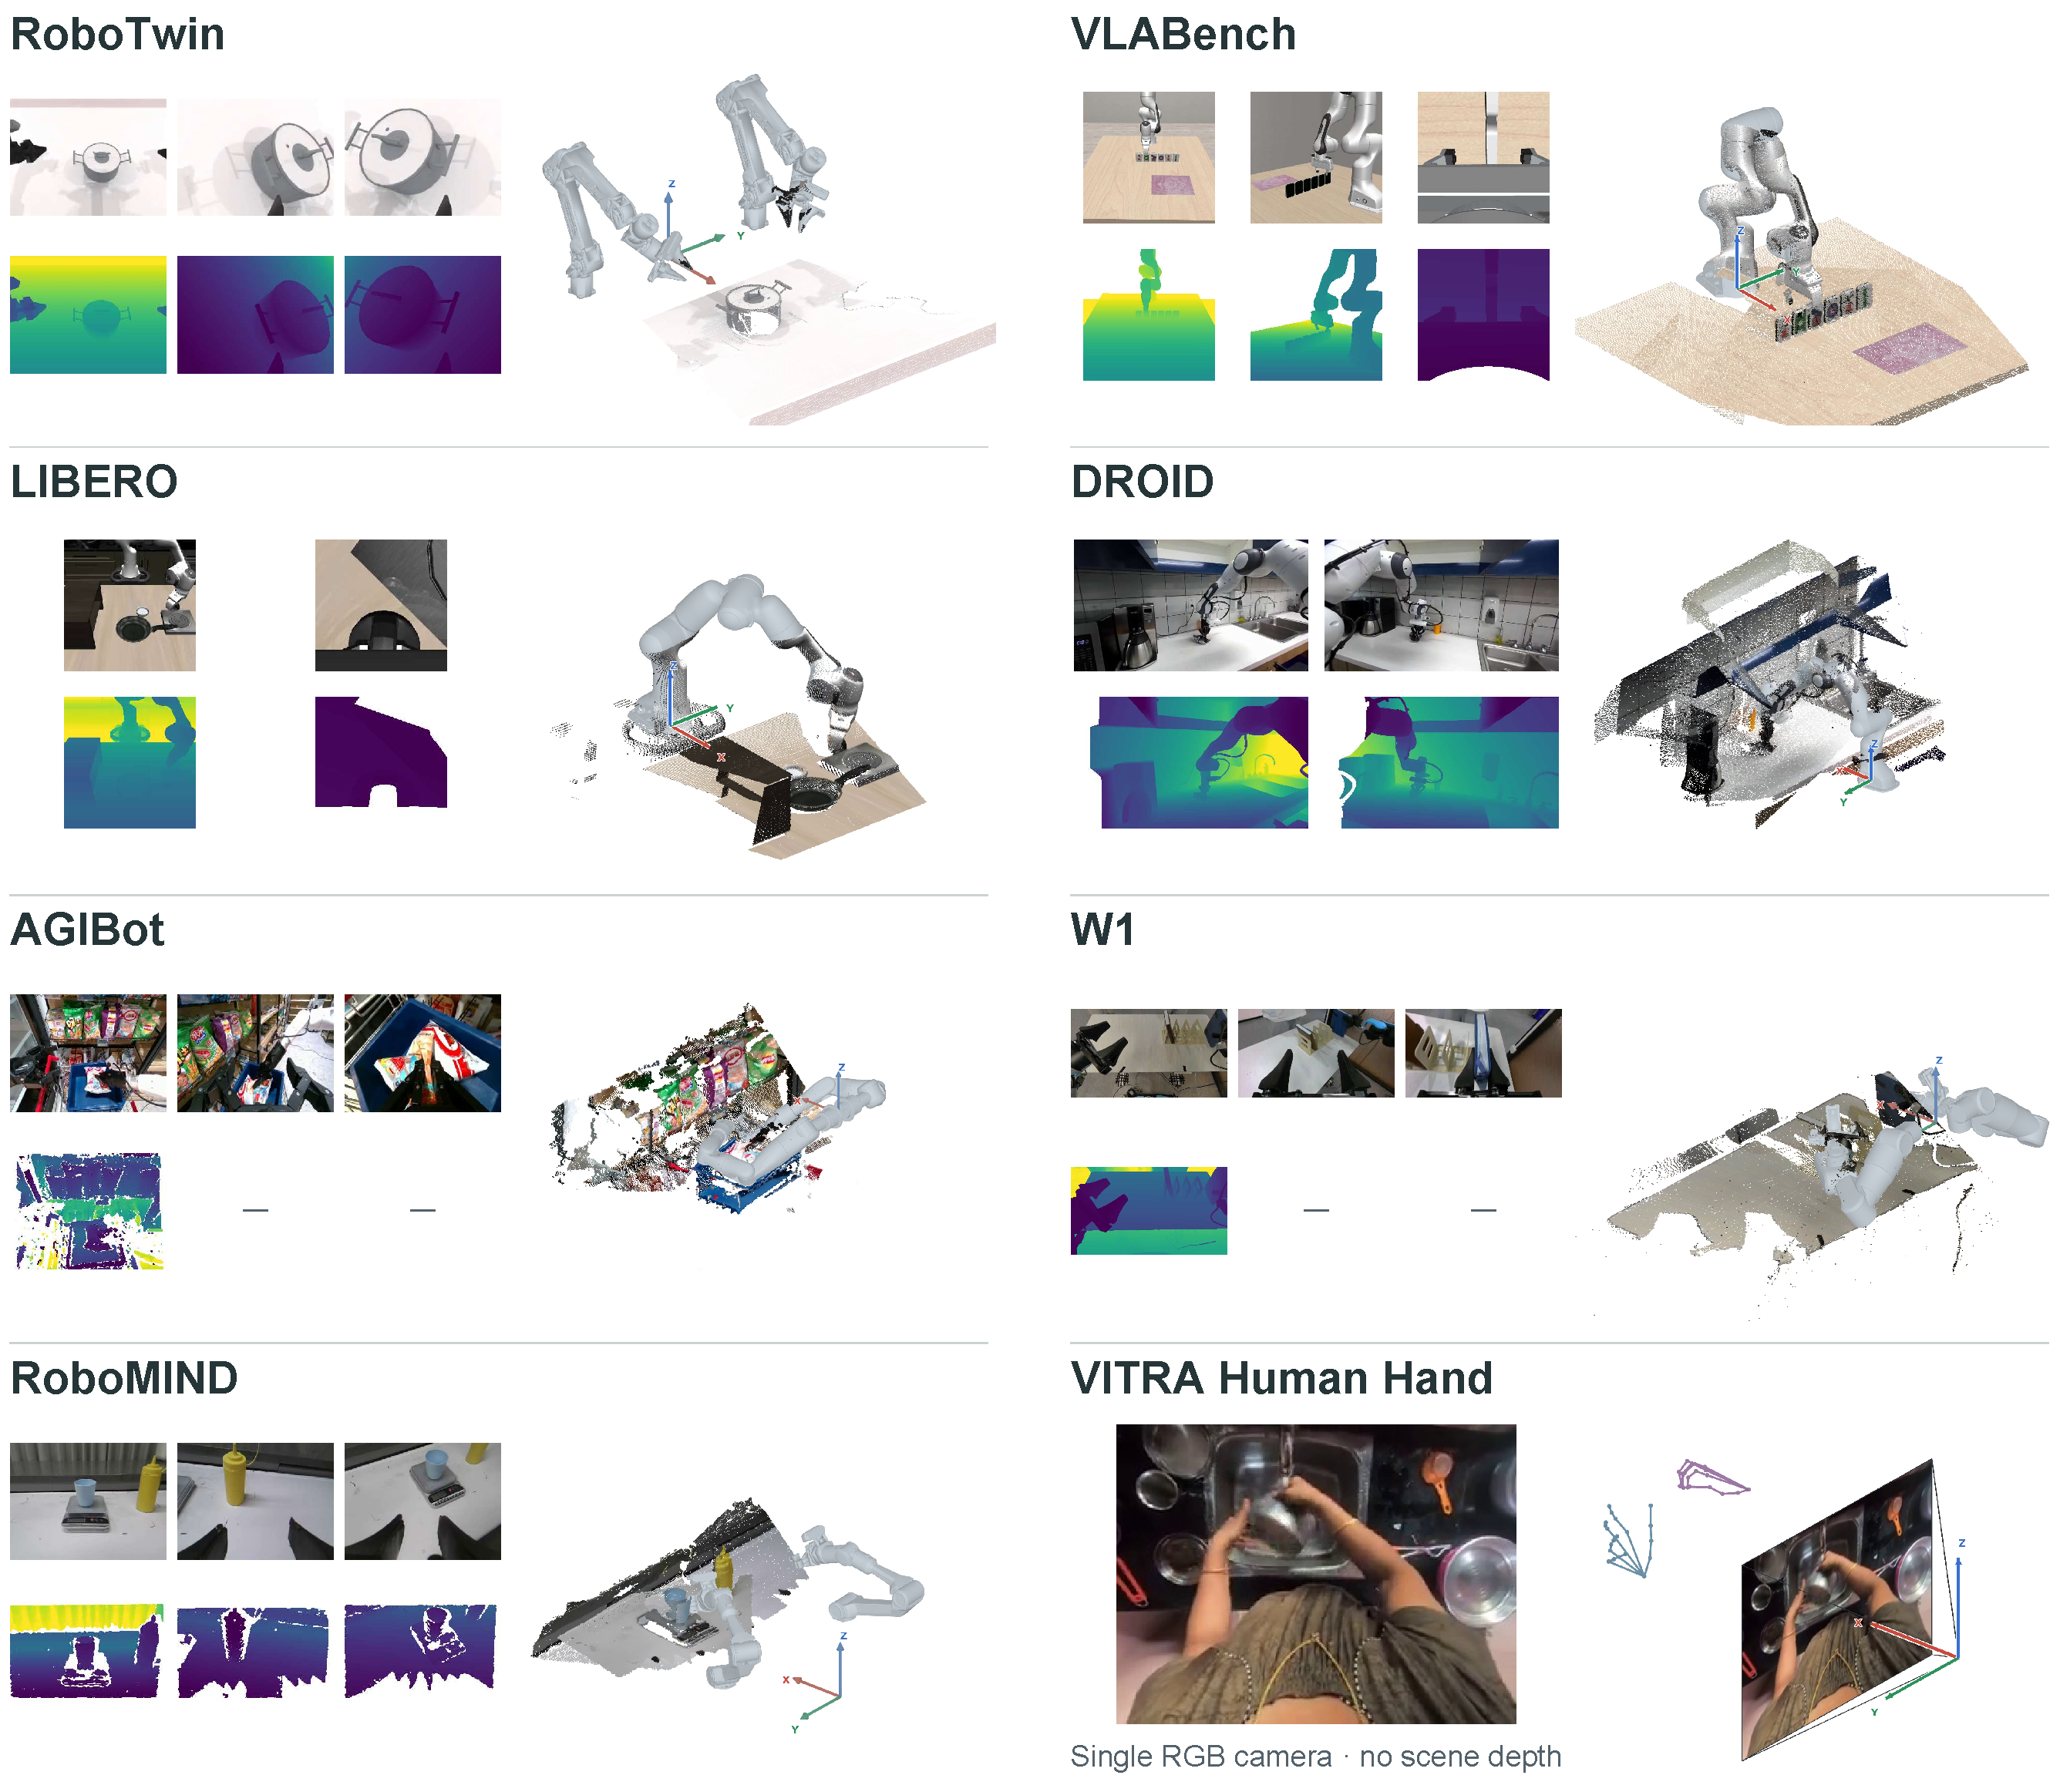
\includegraphics[width=\linewidth]{figures/pretraining_datasets.pdf}
    \caption{\textbf{Representative observations and aligned geometry from
    pretraining data.} Robot panels show RGB, depth where available, and
    scene points with robot overlays. VITRA shows egocentric RGB and hand
    landmarks.}
    \label{fig:app:dataset_visualization}
\end{figure}

\paragraph{Dataset-specific coordinate conventions.}
Robot data use a base or shared embodiment frame. Where specified by the
bimanual adapter, the origin is the arm-base midpoint, with orientation
inherited from the shared root or torso. W1 training coordinates are
centered at the median end-effector trajectory midpoint. For VITRA,
source camera poses transform hand positions into the current anchor's
camera frame, held fixed throughout the window, with
$(x_M,y_M,z_M)=(z_C,-x_C,-y_C)$.

\paragraph{Temporal sampling.}
Tab.~\ref{tab:app:temporal} reports the trajectory sampling settings of
pretraining. The effective sampling rate $f$ accounts for temporal
subsampling: $H$ future intervals span $H/f$ seconds and yield $H+1$
coordinates including the current anchor. We observe slower robot motion
in AgiBot and RoboMIND and therefore
subsample their 45-Hz trajectories with stride 3 (15 Hz). This extends
the physical time covered by each action chunk, bringing its spatial
motion extent closer to that of chunks from the other datasets.
VITRA uses 6 Hz for Ego4D, 8 Hz for EgoExo4D and Something-Something V2,
and 10 Hz for EPIC-KITCHENS. $H_{\mathrm{hist}}$ specifies the data history
window.

\begin{table}[!htbp]
    \centering
    \small
    \setlength{\tabcolsep}{5pt}
    \renewcommand{\arraystretch}{1.12}
    \caption{Pretraining trajectory sampling configuration. $H$ and
    $H_{\mathrm{hist}}$ count future and historical intervals; duration is
    $H/f$ in seconds. $H+1$ includes the current anchor.}
    \label{tab:app:temporal}
    \vspace{3pt}
    \begin{tabular}{@{}llccccc@{}}
        \toprule
        Dataset & Source & $f$ (Hz) & $H$ & $H_{\mathrm{hist}}$ & Duration & $H+1$ \\
        \midrule
        RoboTwin & Simulation & 15 & 20 & 20 & 1.33 & 21 \\
        LIBERO & Simulation & 20 & 20 & 20 & 1.00 & 21 \\
        VLABench & Simulation & 10 & 15 & 15 & 1.50 & 16 \\
        DROID & Real robot & 15 & 20 & 20 & 1.33 & 21 \\
        AgiBot & Real robot & 15 & 20 & 20 & 1.33 & 21 \\
        RoboMIND & Real robot & 15 & 20 & 20 & 1.33 & 21 \\
        RH20T & Real robot & 20 & 20 & 20 & 1.00 & 21 \\
        W1-data & Real robot & 15 & 20 & 20 & 1.33 & 21 \\
        VITRA & Human hand & 6/8/10 & 10 & 10 & $10/f$ & 11 \\
        \bottomrule
    \end{tabular}
\end{table}

\subsection{Physical-Time Trajectory Tokenizer}
\label{app:trajectory_tokenizer}

The encoder and decoder are defined in
Eq.~\eqref{eq:physical_time_flowchunk}.
The temporal basis takes timestamps in seconds on the shared scale
$T_{\max}=3\,\mathrm{s}$:
\begin{equation}
    [\boldsymbol\phi_{\mathrm{time}}(\tau)]_j
    =\operatorname{sgn}(\tau)\,
    \sin\!\left[\frac{\pi}{2}
    \left|\frac{\tau}{T_{\max}}\right|^{j/d_z}\right],
    \qquad j=0,\ldots,d_z-1,
\label{eq:tokenizer_time_basis}
\end{equation}
with latent dimension $d_z=256$.
Future trajectories use positive offsets; history uses negative offsets
and displacements from past positions toward the current anchor.
An input MLP produces $\mathbf h_{n,k}$ from $\Delta\mathbf x_{n,k}$, and
separate temporal MLPs produce the encoder and decoder FiLM parameters.

\paragraph{Reconstruction training.}
We minimize squared Euclidean error over valid point--time pairs,
averaging the future and historical action losses and adding available
scene reconstruction loss. The trained tokenizer is frozen, and its
latents are standardized with fixed channelwise training statistics
before world-action model training.

\paragraph{Spatial anchoring and query sets.}
The spatial anchor is separate from the displacement latent. Pointwise
Fourier features of $\mathbf x_{t,n}$ are projected to the point dynamics expert's
hidden dimension and added to the trajectory token throughout denoising.
Shared token processing and order-independent attention masks make
prediction permutation equivariant within each query type: reordering
query points and their noise tokens together reorders the outputs.
Variable query counts support sparse object-level prediction or denser
scene coverage.


\paragraph{Held-out trajectory reconstruction.}
We evaluate the frozen tokenizer on 600 held-out trajectory windows per
source and trajectory type, none used for tokenizer training. Each point
trajectory is encoded into one token and decoded at its original physical
timestamps. Tab.~\ref{tab:app:tokenizer_reconstruction} reports ADE,
the mean Euclidean error across future timesteps, and FDE, the error at
the final timestep, averaged over point trajectories. The millimeter-scale
errors indicate that the tokenizer preserves motion information across
robot action flow, human-hand action flow, and scene flow in these samples.

\begin{center}
\begin{minipage}{0.805\linewidth}
    \makeatletter\def\@captype{table}\makeatother
    \centering
    \small
    \setlength{\tabcolsep}{6pt}
    \renewcommand{\arraystretch}{1.12}
    \caption{Held-out trajectory reconstruction errors of the frozen
    \mbox{tokenizer} (mm). Dashes indicate unavailable scene-flow ground truth.}
    \label{tab:app:tokenizer_reconstruction}
    \begin{tabular*}{\linewidth}{@{\extracolsep{\fill}}lcccc@{}}
        \toprule
        \multirow{2}{*}{Data source}
        & \multicolumn{2}{c}{Action flow} & \multicolumn{2}{c}{Scene flow} \\
        \cmidrule(lr){2-3}\cmidrule(lr){4-5}
        & ADE $\downarrow$ & FDE $\downarrow$
        & ADE $\downarrow$ & FDE $\downarrow$ \\
        \midrule
        RoboTwin & 1.96 & 4.62 & 1.01 & 2.32 \\
        LIBERO & 2.54 & 6.05 & 0.78 & 1.56 \\
        VLABench & 3.38 & 6.25 & 0.94 & 1.89 \\
        DROID & 3.17 & 7.85 & -- & -- \\
        AgiBot & 2.26 & 4.62 & -- & -- \\
        RoboMIND & 3.48 & 7.60 & -- & -- \\
        RH20T & 3.16 & 4.91 & -- & -- \\
        W1 & 1.70 & 3.33 & -- & -- \\
        VITRA (human hand) & 4.68 & 8.18 & -- & -- \\
        \bottomrule
    \end{tabular*}
\end{minipage}
\end{center}

\noindent\begin{minipage}{\linewidth}
\subsection{Architecture and Optimization}
\label{app:implementation}

Tab.~\ref{tab:app:architecture} summarizes the model configuration.

\begin{center}
    \makeatletter\def\@captype{table}\makeatother
    \centering
    \small
    \setlength{\tabcolsep}{6pt}
    \renewcommand{\arraystretch}{1.12}
    \caption{Model architecture. Parameter counts include the frozen tokenizer.}
    \label{tab:app:architecture}
    \begin{tabular}{@{}llr@{}}
        \toprule
        Component & Configuration & Params. (M) \\
        \midrule
        VLM & Florence-2-large & 570.7 \\
        Point dynamics expert & 28 layers; width 1,280; 20 heads & 826.3 \\
        Action expert & 28 layers; width 640; 10 heads & 256.0 \\
        Trajectory tokenizer & Time-conditioned MLPs; latent dim. 256 & 1.9 \\
        Embeddings and projections & Spatial and modality interfaces & 39.7 \\
        \midrule
        Total & & 1,694.5 \\
        \bottomrule
    \end{tabular}
\end{center}
\end{minipage}


\paragraph{Token structure and attention.}
The mask is specified in Sec.~\ref{sec:method:architecture}.
The action expert has the same depth as the dynamics expert and a smaller
hidden dimension, with one noisy command token per future timestep.
Physical execution time $\tau_k$ enters command tokens through FiLM,
separately from the denoising time.

\paragraph{Flow matching and inference.}
The interpolation and the loss weights are given in
Sec.~\ref{sec:method:architecture}.
At inference, action flow and commands use the same Euler schedule for
10 steps. Scene denoising starts from independent noise.

\paragraph{Training configuration.}
We pretrain for 200K steps with a total batch size of 1,024 using AdamW.
The learning rates are $10^{-4}$ for the point dynamics and action experts and
$10^{-5}$ for the VLM, with weight decay $10^{-8}$.
We use constant learning rates after 1,000 steps of linear warmup.
Training uses 64 BW1000\_H DCUs (64\,GiB each) with FSDP.

\paragraph{Queries and objectives.}
Robot grippers use 20 query points sampled from URDF-defined gripper geometry
per arm; human hands use 21 MANO-derived keypoints per observed hand.
Scene points are voxelized and capped at 12,000 before random
subsampling. The mixed-dataset run retains 1\% (approximately 120 scene
queries at the cap), with 5-mm voxels for the simulation datasets.
RGB inputs are resized to $224\!\times\!224$.
The flow-matching weights are set in
Sec.~\ref{sec:method:architecture}; unavailable supervision is masked.
This run uses a frustum-routing substitution probability of 0.1. Action position coordinates are scaled by 10; rotation and gripper
coordinates retain unit scale. Inference uses 10 Euler steps for each
active expert.


\subsection{Inference Efficiency}
\label{app:inference_efficiency}

We measure inference latency on a single NVIDIA GeForce RTX 5090 D.
As shown in Tab.~\ref{tab:app:inference_efficiency}, \method{} directly
produces executable actions without generating action or scene flows
in 55.77\,ms per chunk, providing a $2.20\times$ speedup over jointly
generating actions and action flow. With only 1.7B parameters, this mode
is $2.81\times$ faster than Fast-WAM without video generation and
substantially faster than the joint video--action baselines
Fast-WAM~\citep{yuan2026fastwam} and Motus~\citep{bi2025motus},
supporting low-latency robot control. In world-model mode, the number
of scene queries can be adjusted at inference to match the desired
spatial sampling density and compute budget. Reducing scene queries
from 3,000 to 1,024 lowers joint prediction latency from 561.60\,ms
to 305.49\,ms, allowing a flexible trade-off between scene coverage
and inference cost.


\begin{table}[!htbp]
    \centering
    \small
    \setlength{\tabcolsep}{6pt}
    \renewcommand{\arraystretch}{1.08}
    \caption{\textbf{Inference efficiency on an RTX 5090 D.}
    Latency is measured per prediction chunk; $N_s$ denotes the number
    of scene queries.}
    \label{tab:app:inference_efficiency}
    \begin{tabular}{@{}lrrr@{}}
        \toprule
        Method / output mode & Params (B) & $N_s$ & Latency (ms) \\
        \midrule
        Fast-WAM (w/o video) & 6.0 & -- & 156.81 \\
        Fast-WAM (joint) & 6.0 & -- & 579.79 \\
        Motus & 8.0 & -- & 2,414.90 \\
        \midrule
        \method{}: actions only & 1.7 & -- & 55.77 \\
        \method{}: actions + action flow & 1.7 & -- & 122.51 \\
        \method{}: actions + both flows & 1.7 & 1,024 & 305.49 \\
        \method{}: actions + both flows & 1.7 & 3,000 & 561.60 \\
        \bottomrule
    \end{tabular}
\end{table}



\section{Spatial Grounding without Depth Input}
\label{app:missing_depth}

Candidate depths, the router, and $\mathcal L_{\mathrm{PE}}$ are defined
in Sec.~\ref{sec:method:observation},
Eqs.~\eqref{eq:frustum_routing} and~\eqref{eq:position_distillation}.
During training, routed features occasionally replace depth-derived
features on valid regions, with the substitution rate reported in
Appendix~\ref{app:implementation}.
This section evaluates the router when depth is removed at test time.

\subsection{Evaluation without Depth Input}
\label{app:missing_depth:evaluation}

We evaluate policy execution on LIBERO-Plus at 100K training steps,
without mixed-dataset pretraining or scene-flow supervision.
Tab.~\ref{tab:app:missing_depth} compares routed PE without depth input
against ground-truth depth PE using the same checkpoint, and includes
the no-3D-PE baseline from Tab.~\ref{tab:experiments:libero_plus_ablation}.
Camera calibration and robot-state inputs remain available in all settings.

\begin{table}[!htbp]
    \centering
    \footnotesize
    \setlength{\tabcolsep}{3pt}
    \renewcommand{\arraystretch}{1.15}
    \caption{\textbf{Spatial grounding without depth input on LIBERO-Plus.}
    Success rates (\%, $\uparrow$) over 10,030 episodes. Routed PE and
    ground-truth depth PE use the same checkpoint.}
    \label{tab:app:missing_depth}
    \begin{adjustbox}{max width=\linewidth}
    \begin{tabular}{@{}lrrrrrrrr@{}}
        \toprule
        Visual spatial encoding
        & Camera & Robot & Language & Light & Background & Noise & Layout & Overall \\
        \midrule
        No visual 3D PE
        & 66.73 & 79.29 & 75.21 & 94.57 & 92.19 & 84.13 & 84.46 & 81.35 \\
        Routed PE (no depth)
        & 83.74 & 79.61 & 74.30 & 91.68 & 84.20 & 93.38 & 85.57 & 84.43 \\
        \midrule
        Ground-truth depth PE
        & 84.37 & 79.68 & 74.24 & 91.94 & 85.13 & 93.88 & 85.18 & 84.68 \\
        \bottomrule
    \end{tabular}
    \end{adjustbox}
\end{table}
% Verified full runs: outputs/appendix_missing_depth_20260925/.
% No-PE reference: libero_plus_no_visual_3dpe_step100000_official10030_fast64_20260904.
% Routed / observed depth: libero_distill_estdepth_100k_20260925 /
% libero_distill_gtdepth_100k_20260924; both use the same 100K checkpoint.

\paragraph{Results.}
Without depth input, routed PE achieves 84.43\% overall success,
closely matching the 84.68\% obtained with ground-truth depth PE.
The gap of only 0.25 percentage points supports the effectiveness of
distilling depth-derived spatial information into RGB-conditioned
positional features, preserving policy performance when depth is
unavailable at inference. Compared with removing visual 3D PE, routed
PE improves overall success by 3.08 points, with the largest gains
under camera-viewpoint perturbations and sensor noise.


\section{Detailed LIBERO-Plus Results}
\label{app:libero_plus}

For both training settings, we train \method{} on standard LIBERO demonstrations
and use the same checkpoints as in the LIBERO evaluation to evaluate directly
on LIBERO-Plus. No additional training or adaptation is performed on
LIBERO-Plus; this is an out-of-distribution evaluation.

Tab.~\ref{tab:experiments:libero_plus} breaks down success rates across
all seven perturbation types in LIBERO-Plus~\citep{fei2025liberoplus};
Tab.~\ref{tab:experiments:simulation} reports overall success.
The comparison additionally includes OpenVLA~\citep{kim2024openvla}
and ABot-M0.5~\citep{chen2026abotm05}.

% Score provenance retained for verification; not typeset.
% \paragraph{Reported-score sources.}
% The $\pi_0$ and OpenVLA scores follow \citet{fei2025liberoplus};
% X-VLA, $\pi_{0.5}$, and Cosmos Policy follow
% \citet{zhang2026wamgeneralization}. Fast-WAM and LingBot-VA scores
% follow \citet{huang2026roboharness}, while LaMP and ABot-M0.5 follow
% their respective reports \citep{wang2026lamp,chen2026abotm05}.
% The additional VLA-JEPA, GE-Act, and ABot-M0 overall scores in
% Tab.~\ref{tab:experiments:simulation} follow
% \citet{zhang2026wamgeneralization}.
% 

\begin{table}[!htbp]
    \centering
    \small
    \setlength{\tabcolsep}{3pt}
    \renewcommand{\arraystretch}{1.10}
    \caption{LIBERO-Plus success rates (\%, $\uparrow$) across seven
    perturbation types. Robot denotes initial-state perturbations.}
    \label{tab:experiments:libero_plus}
    \vspace{3pt}
    \begin{adjustbox}{max width=\linewidth}
    \begin{tabular}{@{}lccccccccc@{}}
        \toprule
        Method & Params (B) & Camera & Robot & Language & Light
        & Background & Noise & Layout & Overall \\
        \midrule
        X-VLA & 1 & 23.4 & \underline{89.7} & 75.7 & 88.2 & 96.0 & 62.7 & 71.8 & 71.4 \\
        $\pi_{0}$ & 3 & 13.8 & 6.0 & 58.8 & 85.0 & 81.4 & 79.0 & 68.9 & 53.6 \\
        $\pi_{0.5}$ & 3 & 75.4 & 77.5 & 85.6 & \underline{96.9} & 94.6 & 89.7 & \underline{85.7} & 85.7 \\
        OpenVLA & 7 & 0.8 & 3.5 & 23.0 & 8.1 & 34.8 & 15.2 & 28.5 & 15.6 \\
        Cosmos Policy & 2 & 75.8 & 63.3 & 81.7 & 96.5 & 88.9 & \textbf{92.7} & 82.2 & 82.2 \\
        LingBot-VA & 5.3 & 40.9 & 83.0 & 86.4 & 82.3 & 53.1 & 64.4 & 76.2 & 69.5 \\
        Fast-WAM & 6 & 16.4 & 44.5 & 68.9 & 78.2 & 53.7 & 37.7 & 60.7 & 51.5 \\
        ABot-M0.5 & 6 & 70.5 & 87.4 & \textbf{88.6} & 94.0 & 89.7 & 75.5 & 85.2 & 83.4 \\
        LaMP & 5 & 64.5 & 69.6 & \underline{88.2} & 95.3 & \textbf{97.4} & 76.9 & 73.8 & 79.3 \\
        \midrule
        \method{} (w/o Pretrain) & 1.7 & \underline{81.9} & 84.8 & 77.6 & 96.7 & 94.4 & \underline{89.8} & 85.1 & \underline{86.5} \\
        \method{} & 1.7 & \textbf{82.1} & \textbf{94.2} & 85.0 & \textbf{98.1} & \underline{96.3} & 84.5 & \textbf{87.7} & \textbf{89.1} \\
        \bottomrule
    \end{tabular}
    \end{adjustbox}
\end{table}


\section{Detailed VLABench Results}
\label{app:vlabench}

Tab.~\ref{tab:app:vlabench} reports five evaluation tracks:
in-distribution, cross-category, commonsense, semantic instruction, and
unseen texture (Tracks~1, 2, 3, 4, and 6). The comparison additionally
includes $\pi_0$-FAST~\citep{pertsch2025fast}.

% PhysWAM source: user-provided aggregate evaluation counts.
% Track: N; success count; PS sum; IS sum.
% 1: 500; 310; 382.6667; 401
% 2: 460; 117; 171.1667; 210
% 3: 500; 245; 316.8333; 364
% 4: 500; 312; 379.1667; 399
% 6: 500; 263; 342.6667; 388
% Full method: baidu_edge_04, vlabench_continue200k_to250k_20260920/evaluation/
% model-step-250000; per-episode progress_score/intention_score; valid episodes only.
% Macro SR/PS/IS before rounding: 56.1788649 / 67.5921824 / 69.3225916.
% Baselines: Xiaomi-Robotics-1 (arXiv:2607.15330v1), Table 4;
% Bridge-WA (arXiv:2607.02195), Tables 1 (SR) and 2 (PS/IS).
\begin{center}
\begin{minipage}{\linewidth}
\makeatletter\def\@captype{table}\makeatother
    \centering
    \small
    \setlength{\tabcolsep}{4pt}
    \renewcommand{\arraystretch}{1.15}
    \caption{Detailed VLABench results (\%). SR, PS, and IS denote
    success rate, progress score, and intention score, respectively
    (all $\uparrow$).}
    \label{tab:app:vlabench}
    \vspace{3pt}
    \begin{adjustbox}{max width=\linewidth}
    \begin{tabular*}{0.94\linewidth}{@{\extracolsep{\fill}}l*{9}{r}@{}}
        \toprule
        Method & \multicolumn{3}{c}{In-distribution}
        & \multicolumn{3}{c}{Cross-category}
        & \multicolumn{3}{c}{Commonsense} \\
        \cmidrule(lr){2-4}\cmidrule(lr){5-7}\cmidrule(lr){8-10}
        & SR & PS & IS & SR & PS & IS & SR & PS & IS \\
        \midrule
        $\pi_0$ & 47.0 & 62.7 & 67.8 & 21.2 & 33.6 & 44.0 & 29.1 & 43.0 & 54.9 \\
        $\pi_0$-FAST & 56.2 & 66.8 & 72.4 & \underline{31.0} & 38.2 & \underline{47.8} & 38.0 & 48.6 & 56.8 \\
        X-VLA & 40.0 & 66.5 & \textbf{88.0} & 11.0 & 24.0 & 42.0 & 33.0 & 51.7 & 66.0 \\
        $\pi_{0.5}$ & \underline{65.4} & \underline{77.8} & 80.4 & \textbf{38.2} & \textbf{49.7} & \textbf{52.0} & 43.9 & 57.3 & 60.0 \\
        \midrule
        \method{} (w/o Pretrain) & 62.0 & 76.5 & 80.2 & 25.4 & 37.2 & 45.7 & \underline{49.0} & \underline{63.4} & \textbf{72.8} \\
        \method{} & \textbf{75.1} & \textbf{85.6} & \underline{82.3} & 28.9 & \underline{39.1} & 44.4 & \textbf{53.8} & \textbf{65.9} & \underline{68.5} \\
        \midrule
        Method & \multicolumn{3}{c}{Semantic instruction}
        & \multicolumn{3}{c}{Unseen texture}
        & \multicolumn{3}{c}{Avg.} \\
        \cmidrule(lr){2-4}\cmidrule(lr){5-7}\cmidrule(lr){8-10}
        & SR & PS & IS & SR & PS & IS & SR & PS & IS \\
        \midrule
        $\pi_0$ & 17.3 & 38.7 & 58.0 & 32.2 & 42.5 & 50.6 & 29.4 & 44.1 & 55.0 \\
        $\pi_0$-FAST & 35.0 & 45.0 & 59.4 & 39.0 & 49.0 & 56.8 & 39.8 & 49.5 & 58.6 \\
        X-VLA & 39.0 & 62.5 & \textbf{82.0} & 24.0 & 51.2 & \underline{73.0} & 29.4 & 51.2 & \underline{70.2} \\
        $\pi_{0.5}$ & 48.2 & 64.2 & 67.0 & 44.9 & 62.3 & 65.0 & 48.1 & 62.3 & 64.9 \\
        \midrule
        \method{} (w/o Pretrain) & \underline{62.4} & \underline{75.8} & \underline{79.8} & \underline{52.6} & \textbf{68.5} & \textbf{77.6} & \underline{50.3} & \underline{64.3} & \textbf{71.2} \\
        \method{} & \textbf{67.7} & \textbf{79.9} & 78.7 & \textbf{55.4} & \underline{67.4} & 72.7 & \textbf{56.2} & \textbf{67.6} & 69.3 \\
        \bottomrule
    \end{tabular*}
    \end{adjustbox}
\end{minipage}
\end{center}


\section{Detailed RoboTwin Results}
\label{app:robotwin}

Tab.~\ref{tab:app:robotwin} gives per-task results for both training settings
in Tab.~\ref{tab:experiments:simulation}. Each setting contains 50 tasks
with 100 evaluation episodes per task; averages weight all tasks equally.

% Table values confirmed as updated by the author on 2026-09-24.
\begin{center}
\begin{minipage}{\linewidth}
\makeatletter\def\@captype{table}\makeatother
    \centering
    \fontsize{8}{9}\selectfont
    \setlength{\tabcolsep}{3pt}
    \renewcommand{\arraystretch}{0.98}
    \caption{Detailed RoboTwin 2.0 success rates (\%, $\uparrow$).
    Clean and Rand.\ denote \texttt{demo\_clean} and \texttt{demo\_randomized}.
    All methods are evaluated over 100 episodes per task in each setting.}
    \label{tab:app:robotwin}
    \vspace{3pt}
    \begin{tabular*}{\linewidth}{@{\extracolsep{\fill}}l*{10}{c}@{}}
        \toprule
        Task & \multicolumn{2}{c}{$\pi_{0.5}$}
        & \multicolumn{2}{c}{Motus} & \multicolumn{2}{c}{Fast-WAM}
        & \multicolumn{2}{c}{\shortstack{\method{}\\(w/o Pretrain)}}
        & \multicolumn{2}{c}{\method{}} \\
        \cmidrule(lr){2-3}\cmidrule(lr){4-5}\cmidrule(lr){6-7}
        \cmidrule(lr){8-9}\cmidrule(lr){10-11}
        & Clean & Rand. & Clean & Rand. & Clean & Rand.
        & Clean & Rand. & Clean & Rand. \\
        \midrule
        Adjust Bottle & \textbf{100} & \underline{99} & \underline{89} & 93 & \textbf{100} & \textbf{100} & \textbf{100} & 98 & \textbf{100} & \textbf{100} \\
        Beat Block Hammer & 96 & 93 & 95 & 88 & \underline{99} & \underline{97} & 97 & 92 & \textbf{100} & \textbf{98} \\
        Blocks Ranking RGB & 92 & 85 & \underline{99} & 97 & \textbf{100} & \textbf{100} & \textbf{100} & \underline{99} & 97 & 94 \\
        Blocks Ranking Size & 49 & 26 & 75 & 63 & \textbf{94} & \textbf{98} & \underline{91} & \underline{83} & 78 & 82 \\
        Click Alarmclock & \underline{98} & \underline{89} & \textbf{100} & \textbf{100} & \textbf{100} & \textbf{100} & \textbf{100} & \textbf{100} & \textbf{100} & \textbf{100} \\
        Click Bell & \underline{99} & \underline{66} & \textbf{100} & \textbf{100} & \textbf{100} & \textbf{100} & \textbf{100} & \textbf{100} & \textbf{100} & \textbf{100} \\
        Dump Bin Bigbin & 92 & \underline{97} & 95 & 91 & \underline{97} & 96 & \underline{97} & \textbf{98} & \textbf{98} & \underline{97} \\
        Grab Roller & \textbf{100} & \textbf{100} & \textbf{100} & \textbf{100} & \textbf{100} & \textbf{100} & \textbf{100} & \textbf{100} & \textbf{100} & \textbf{100} \\
        Handover Block & 66 & 57 & 86 & 73 & \underline{95} & \underline{81} & 88 & 74 & \textbf{96} & \textbf{84} \\
        Handover Mic & 98 & 97 & 78 & 63 & \underline{99} & \textbf{100} & \textbf{100} & \underline{99} & \textbf{100} & 97 \\
        Hanging Mug & 18 & 17 & 38 & 38 & \underline{58} & \textbf{62} & 48 & \underline{57} & \textbf{61} & 41 \\
        Lift Pot & 96 & 85 & 96 & \underline{99} & \textbf{100} & \textbf{100} & 98 & \underline{99} & \underline{99} & \underline{99} \\
        Move Can Pot & 51 & 55 & 34 & 74 & 90 & 88 & \textbf{97} & \textbf{100} & \underline{94} & \underline{96} \\
        Move Pillbottle Pad & 84 & 61 & 93 & 96 & \textbf{100} & \textbf{99} & \underline{99} & \textbf{99} & 93 & \underline{98} \\
        Move Playingcard Away & 96 & 84 & \textbf{100} & \underline{96} & \textbf{100} & \textbf{100} & \underline{98} & \textbf{100} & \textbf{100} & \textbf{100} \\
        Move Stapler Pad & 56 & 42 & \textbf{83} & \textbf{85} & 77 & 64 & 54 & 50 & \underline{79} & \underline{78} \\
        Open Laptop & 90 & 96 & 95 & 91 & \underline{98} & \textbf{100} & \underline{98} & \underline{99} & \textbf{100} & \textbf{100} \\
        Open Microwave & 34 & 77 & \underline{95} & \textbf{91} & 62 & 45 & \textbf{96} & \underline{86} & 74 & 80 \\
        Pick Diverse Bottles & 81 & 71 & \textbf{90} & \textbf{91} & 80 & 85 & 84 & 81 & \underline{86} & \underline{88} \\
        Pick Dual Bottles & 93 & 63 & \underline{96} & 90 & \textbf{100} & \underline{96} & \underline{96} & \textbf{98} & \textbf{100} & \textbf{98} \\
        Place A2B Left & 87 & 82 & 88 & 79 & \underline{95} & 93 & 90 & \underline{95} & \textbf{100} & \textbf{98} \\
        Place A2B Right & 87 & 84 & 91 & 87 & \textbf{93} & \textbf{99} & \underline{92} & 95 & \textbf{93} & \underline{98} \\
        Place Bread Basket & 77 & 64 & \underline{91} & \underline{94} & \underline{91} & 93 & \textbf{95} & \textbf{98} & \textbf{95} & 91 \\
        Place Bread Skillet & 85 & 66 & 86 & 83 & \textbf{90} & \underline{93} & 87 & \textbf{95} & \underline{89} & 86 \\
        Place Burger Fries & 94 & 87 & \underline{98} & \underline{98} & 96 & \textbf{99} & \textbf{100} & \textbf{99} & 96 & \underline{98} \\
        Place Can Basket & 62 & 62 & \textbf{81} & \underline{76} & 71 & 69 & 72 & 74 & \underline{77} & \textbf{92} \\
        Place Cans Plasticbox & 94 & 84 & \underline{98} & 94 & \textbf{99} & 96 & \textbf{99} & \underline{97} & \textbf{99} & \textbf{99} \\
        Place Container Plate & \underline{99} & 95 & 98 & \underline{99} & 96 & \textbf{100} & \underline{99} & 95 & \textbf{100} & \underline{99} \\
        Place Dual Shoes & 75 & 75 & 93 & 87 & \underline{94} & 88 & 92 & \underline{91} & \textbf{99} & \textbf{96} \\
        Place Empty Cup & \textbf{100} & \underline{99} & \underline{99} & 98 & \textbf{100} & \textbf{100} & \textbf{100} & \textbf{100} & \textbf{100} & \textbf{100} \\
        Place Fan & 87 & 85 & \underline{91} & 87 & \textbf{96} & \textbf{96} & 89 & 92 & 90 & \underline{94} \\
        Place Mouse Pad & 60 & 39 & 66 & 68 & 83 & \underline{89} & \underline{89} & \textbf{92} & \textbf{91} & 87 \\
        Place Object Basket & 80 & 76 & 81 & 87 & \underline{89} & 88 & 79 & \textbf{94} & \textbf{94} & \underline{91} \\
        Place Object Scale & 86 & 80 & 88 & 85 & \underline{90} & \textbf{97} & \textbf{91} & \underline{94} & \textbf{91} & 91 \\
        Place Object Stand & 91 & 85 & \textbf{98} & \textbf{97} & 90 & \underline{94} & 92 & 88 & \underline{97} & \textbf{97} \\
        Place Phone Stand & 81 & 81 & 87 & 86 & \textbf{97} & \textbf{99} & 85 & 89 & \underline{89} & \underline{95} \\
        Place Shoe & 92 & 93 & \underline{99} & 97 & 96 & \textbf{99} & 97 & 97 & \textbf{100} & \underline{98} \\
        Press Stapler & 87 & 83 & \underline{93} & \textbf{98} & 90 & \underline{97} & \textbf{98} & \textbf{98} & \textbf{98} & 96 \\
        Put Bottles Dustbin & 84 & 79 & 81 & 79 & \textbf{95} & \underline{90} & \underline{87} & \underline{90} & 85 & \textbf{98} \\
        Put Object Cabinet & 80 & 79 & \underline{88} & 71 & \textbf{94} & \underline{89} & \underline{88} & 84 & 77 & \textbf{92} \\
        Rotate QR Code & 89 & 87 & 89 & 73 & \textbf{93} & 89 & 91 & \underline{91} & \underline{92} & \textbf{92} \\
        Scan Object & 72 & 65 & 67 & 66 & \underline{89} & \underline{92} & 87 & \underline{92} & \textbf{97} & \textbf{96} \\
        Shake Bottle & \underline{99} & 97 & \textbf{100} & 97 & \textbf{100} & \textbf{100} & \textbf{100} & 97 & \textbf{100} & \underline{99} \\
        Shake Bottle Horizontally & \underline{99} & \underline{99} & \textbf{100} & 98 & \textbf{100} & \textbf{100} & \textbf{100} & 94 & \textbf{100} & \textbf{100} \\
        Stack Blocks Three & 91 & 76 & 91 & \underline{95} & \underline{95} & \textbf{97} & 93 & 84 & \textbf{98} & 94 \\
        Stack Blocks Two & 97 & \textbf{100} & \textbf{100} & \underline{98} & \textbf{100} & \textbf{100} & \underline{99} & \underline{98} & \textbf{100} & 96 \\
        Stack Bowls Three & 77 & 71 & 79 & \textbf{87} & \underline{80} & 81 & \textbf{84} & \textbf{87} & \textbf{84} & \underline{85} \\
        Stack Bowls Two & \underline{95} & 96 & \textbf{98} & 98 & 92 & 98 & 91 & \underline{99} & \underline{95} & \textbf{100} \\
        Stamp Seal & 79 & 55 & \textbf{93} & \underline{92} & \underline{90} & \textbf{94} & 79 & 63 & 83 & \underline{92} \\
        Turn Switch & 62 & 54 & \textbf{84} & \textbf{78} & 61 & 59 & 68 & 63 & \underline{83} & \underline{72} \\
        \midrule
        Average & 82.74 & 76.76 & 88.66 & 87.02 & \underline{91.88} & \underline{91.78} & 91.08 & 90.74 & \textbf{92.94} & \textbf{93.04} \\
        \bottomrule
    \end{tabular*}
\end{minipage}
\end{center}


\section{World Model Evaluation Details}
\label{app:world_model_protocol}

\subsection{Action-Conditioned Scene Prediction}
\label{app:matched_action}

\paragraph{Evaluation protocol.}
Tab.~\ref{tab:experiments:world_model} evaluates 550 test clips from
50 RoboTwin tasks, with one Clean and ten Randomized episodes per task.
Each episode contributes a fixed window near its midpoint, containing
the current frame and 20 future recorded frames. Initial scene points
are sampled with a 1.5\,cm voxel grid.
All methods share initial queries, point identities, ground-truth
trajectories, and robot-motion conditions.
For video methods, queries are projected into the initial image using camera calibration,
accounting for resizing and cropping; only in-frame projections are
tracked by SpatialTrackerV2. Ctrl-World uses Depth Anything 3 depth,
whereas X-WAM uses its native depth predictions. Depth scale for
Ctrl-World and inverse-depth affine calibration for X-WAM are estimated
from initial observed depth and fixed throughout the video. Tracked
trajectories are transformed into world coordinates, and their predicted
displacements are anchored at the shared initial queries. No future
ground-truth depth or trajectories are used for alignment.

\paragraph{Scoring.}
In our evaluation, we label a point as moving when its maximum
ground-truth displacement from its initial position over the 20 future
frames exceeds 1\,cm, and as static otherwise. These labels are fixed
per clip and shared across methods. We score future frames $4,8,12,16,20$: ADE averages Euclidean
errors over valid point--frame pairs in each group, Moving FDE measures
moving-point error at frame 20, and Moving Acc@1cm is the fraction of
valid moving-point--frame pairs with prediction error at most 1\,cm.
Metrics are first computed per clip, averaged within each task--condition
group, and then averaged equally across groups. Clips without valid
moving points are excluded only from the corresponding moving metrics.

\subsection{Closed-Loop Action--Scene Consistency}
\label{app:future_action_alignment}

We evaluate three RoboTwin tasks, Adjust Bottle, Beat Block Hammer, and
Blocks Ranking RGB, under Clean and Randomized conditions, yielding six
settings. Each method is evaluated over 10 trials per setting, for 60
trials in total. We compare with X-WAM~\citep{guo2026xwam},
Fast-WAM~\citep{yuan2026fastwam}, LingBot-VA~\citep{li2026lingbotva},
and Motus~\citep{bi2025motus}. Each generated action chunk is executed
in the simulator, and the resulting observation conditions the next
prediction. Models retain their native prediction horizons and are
scored at completed action boundaries until termination. Fast-WAM
executes all 32 actions rather than replanning after 24.
% Native action/future-frame counts: X-WAM32/8, Fast-WAM32/8,
% LingBot16/4 then32/8, Motus16/8, Unitas20/20.

For \method{}, the point dynamics expert generates an action flow, while the action
expert separately generates an executable command chunk from the same
observation and instruction. The dynamics expert then predicts scene-flow
trajectories conditioned on its generated action flow. We compare these
predictions with the ground-truth scene trajectories resulting from
executing the action expert's command chunk in the simulator.

\paragraph{Trajectory extraction and scoring.}
Ground-truth query points follow their simulator objects or links.
SpatialTrackerV2 lifts video predictions using X-WAM's native depth or
Depth Anything 3 estimates for RGB-only models, with initial-frame depth
calibration and query anchoring. We apply the 1\,cm displacement threshold
to label moving points within each scored chunk. Metrics are averaged
within rounds, then within episodes, across trials within each setting,
and finally equally across the six settings. Rounds without valid moving points are excluded only from
moving-point metrics; all episodes are retained regardless of task outcome.

\begin{center}
\begin{minipage}{\linewidth}
\makeatletter\def\@captype{table}\makeatother
    \centering
    \small
    \setlength{\tabcolsep}{4pt}
    \renewcommand{\arraystretch}{1.10}
    \caption{\textbf{Closed-loop action--scene consistency on RoboTwin.}
    Predictions are compared with the scene evolution produced by executing
    the same model's generated actions. Errors are in cm; Moving Acc@1cm
    is in \%.}
    \label{tab:app:joint_consistency}
    \begin{adjustbox}{max width=\linewidth}
    \begin{tabular}{@{}lcccc@{}}
        \toprule
        Method & Moving ADE $\downarrow$ & Static ADE $\downarrow$
        & Moving FDE $\downarrow$ & Moving Acc@1cm $\uparrow$ \\
        \midrule
        X-WAM + STv2 & \underline{2.579} & \underline{0.166} & \underline{4.056} & 35.55 \\
        Fast-WAM + STv2 & 3.554 & 0.586 & 5.133 & 30.37 \\
        LingBot-VA + STv2 & 2.603 & 0.810 & 4.716 & 33.64 \\
        Motus + STv2 & 3.216 & 0.318 & 6.778 & \underline{35.66} \\
        \method{} & \textbf{1.211} & \textbf{0.054} & \textbf{2.020} & \textbf{64.26} \\
        \bottomrule
    \end{tabular}
    \end{adjustbox}
\end{minipage}
\end{center}
% Results and independent verification: outputs/wam_final_20260922/.
% PhysWAM updated: DCU3 step292814; outputs/physwam_dcu292814_20260922/.

These scores measure action--scene consistency along each model's own
rollout and include video-to-3D reconstruction error for video-based methods.
For \method{}, agreement between predicted and observed scene changes also
provides indirect evidence that its generated action flow and executable
commands are consistent in their scene effects.


\section{Additional Action-Conditioned Scene Predictions}
\label{app:scene_flow_visualizations}

\subsection{Scene Prediction in Simulation}
\label{app:sim_scene_flow}

Figs.~\ref{fig:app:scene_flow_1}--\ref{fig:app:scene_flow_4} extend
Fig.~\ref{fig:experiments:scene_flow_qualitative} with 19 training clips,
showing RGB, initial points, predicted flows, and ground-truth flows.
Purple denotes conditioning gripper motion. These examples illustrate
learned geometry rather than held-out accuracy. For denser visualization,
we relax part-boundary and depth-jump filters while retaining valid-depth
and non-robot checks. Every displayed scene point is directly predicted;
initial RGB colors are retained and unobserved surfaces are not synthesized.

\begin{center}
\begin{minipage}{\linewidth}
\makeatletter\def\@captype{figure}\makeatother
    \centering
    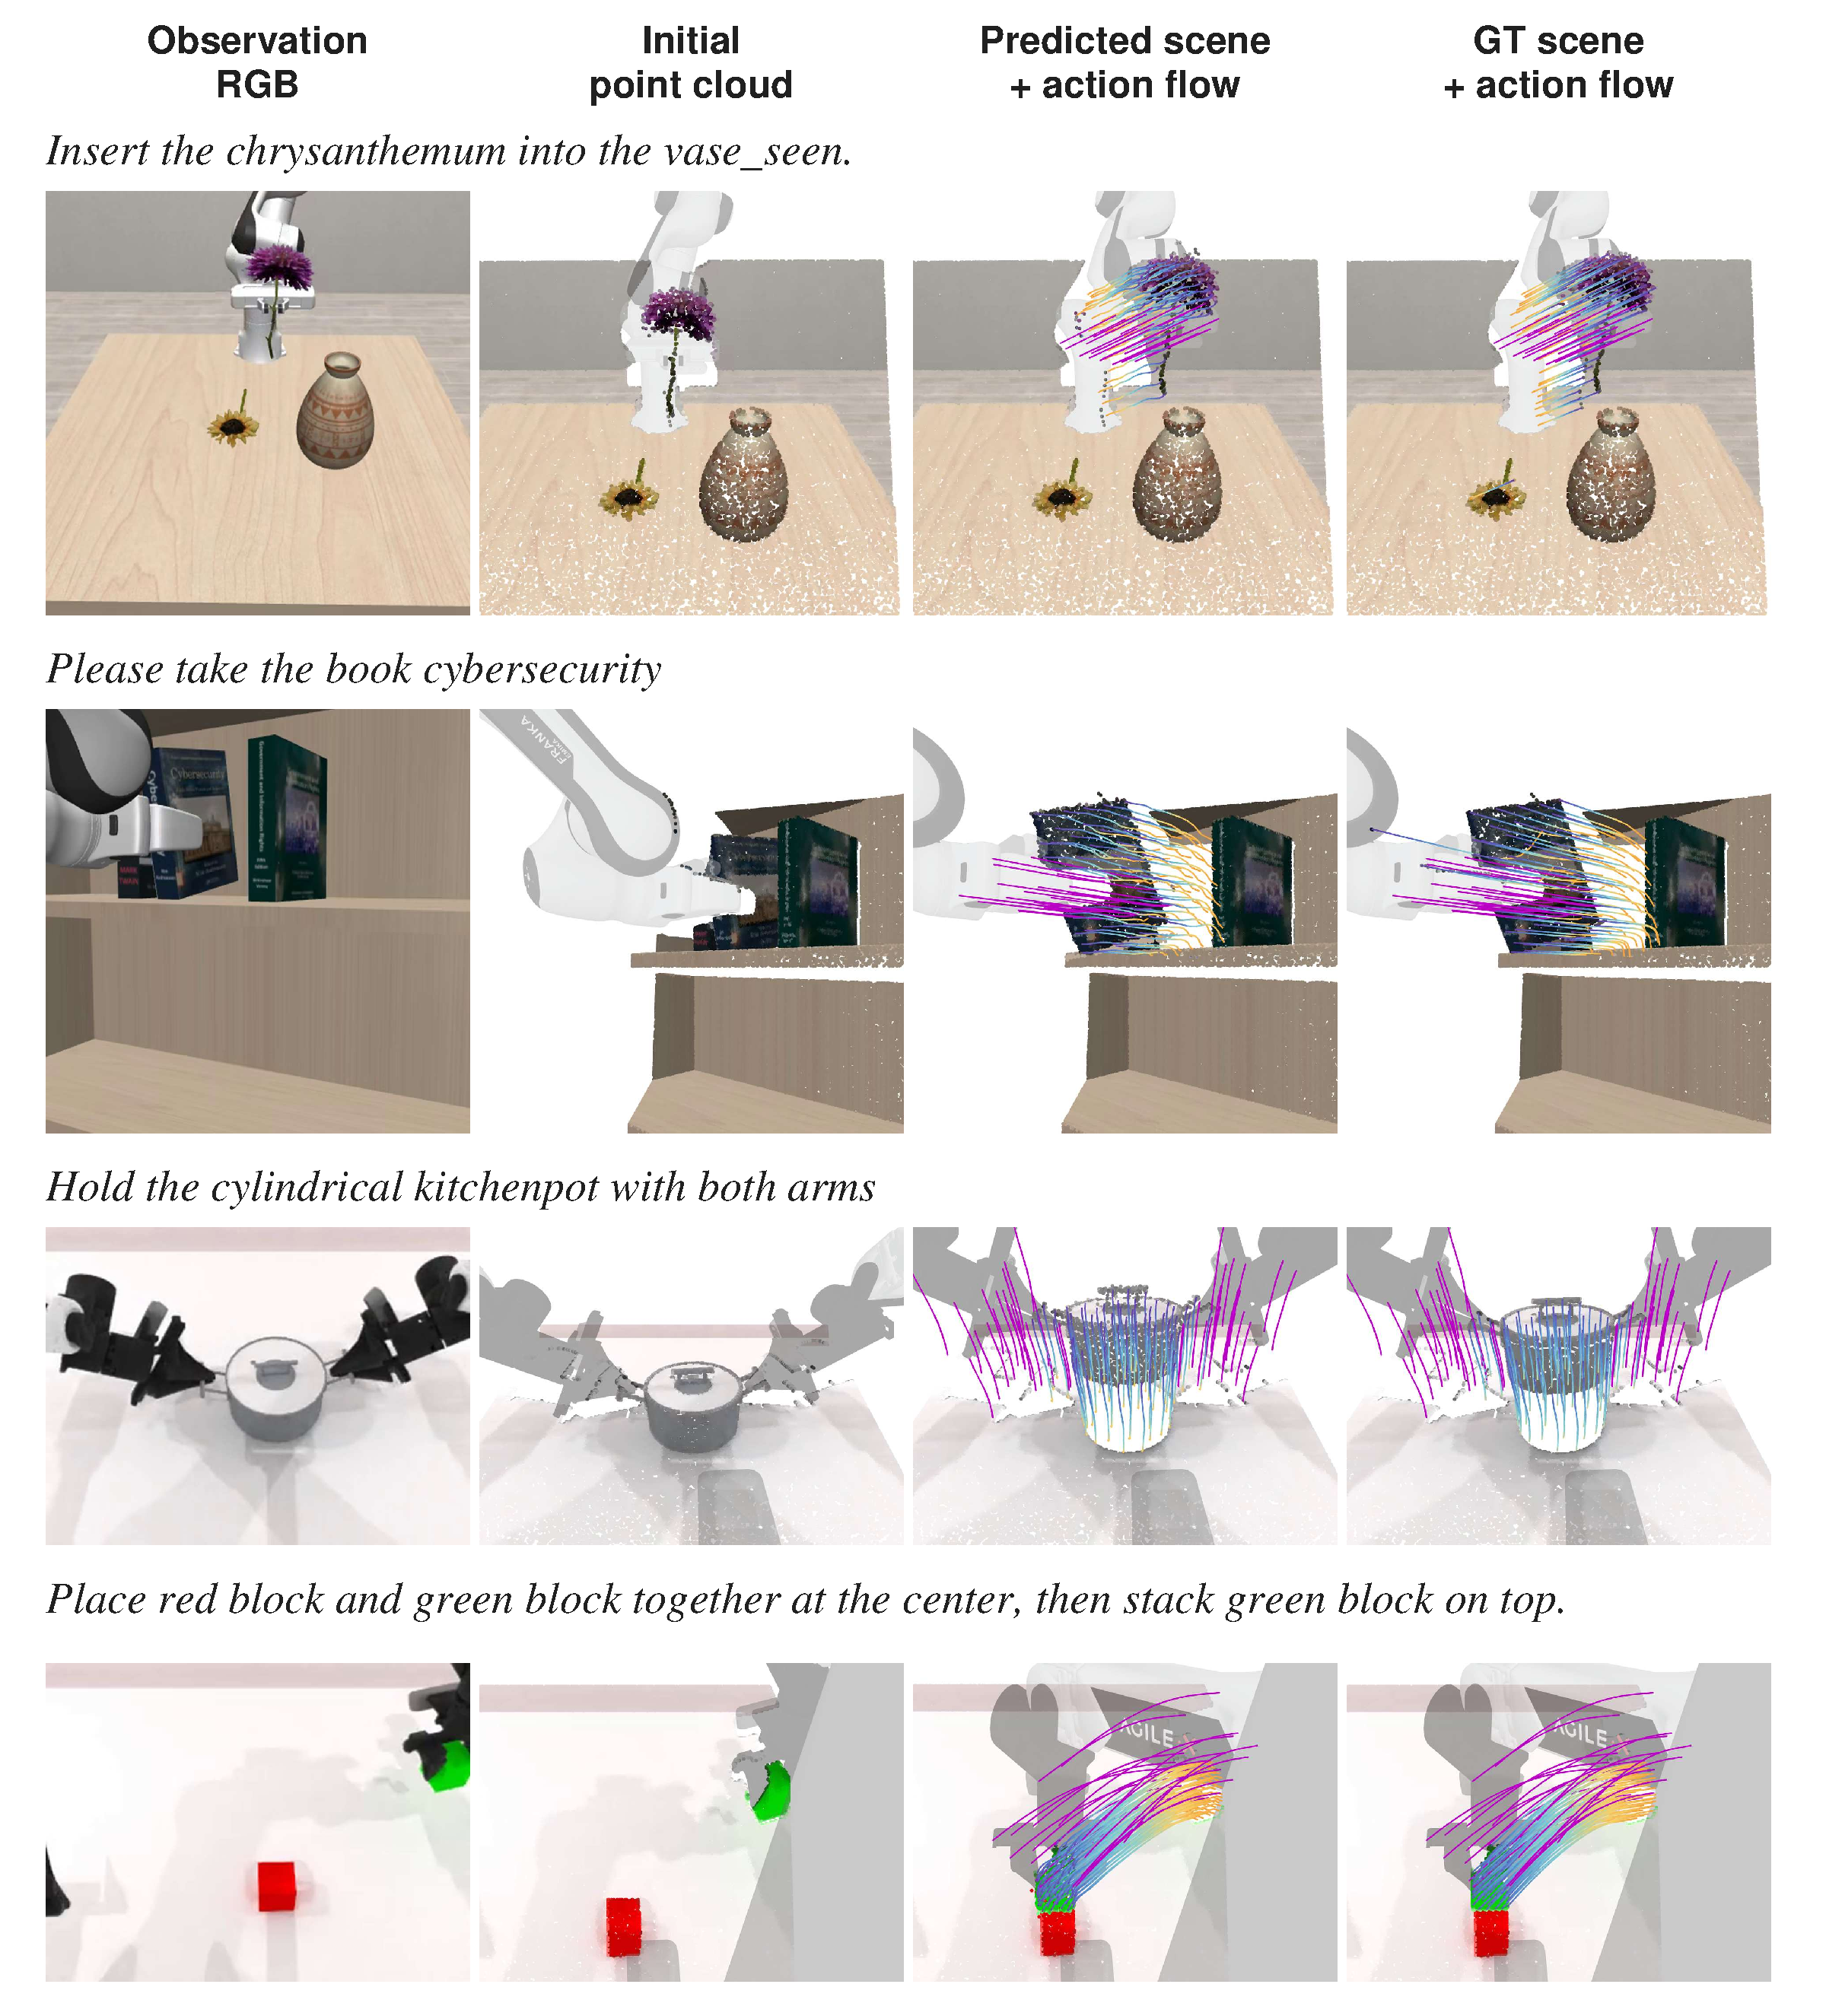
\includegraphics[width=\linewidth]{figures/scene_flow_appendix_1.pdf}
    \caption{Additional scene-flow visualizations (1/4): insertion,
    extraction, bimanual lifting, and block stacking.}
    \label{fig:app:scene_flow_1}
\end{minipage}
\end{center}


\begin{center}
\begin{minipage}{\linewidth}
\makeatletter\def\@captype{figure}\makeatother
    \centering
    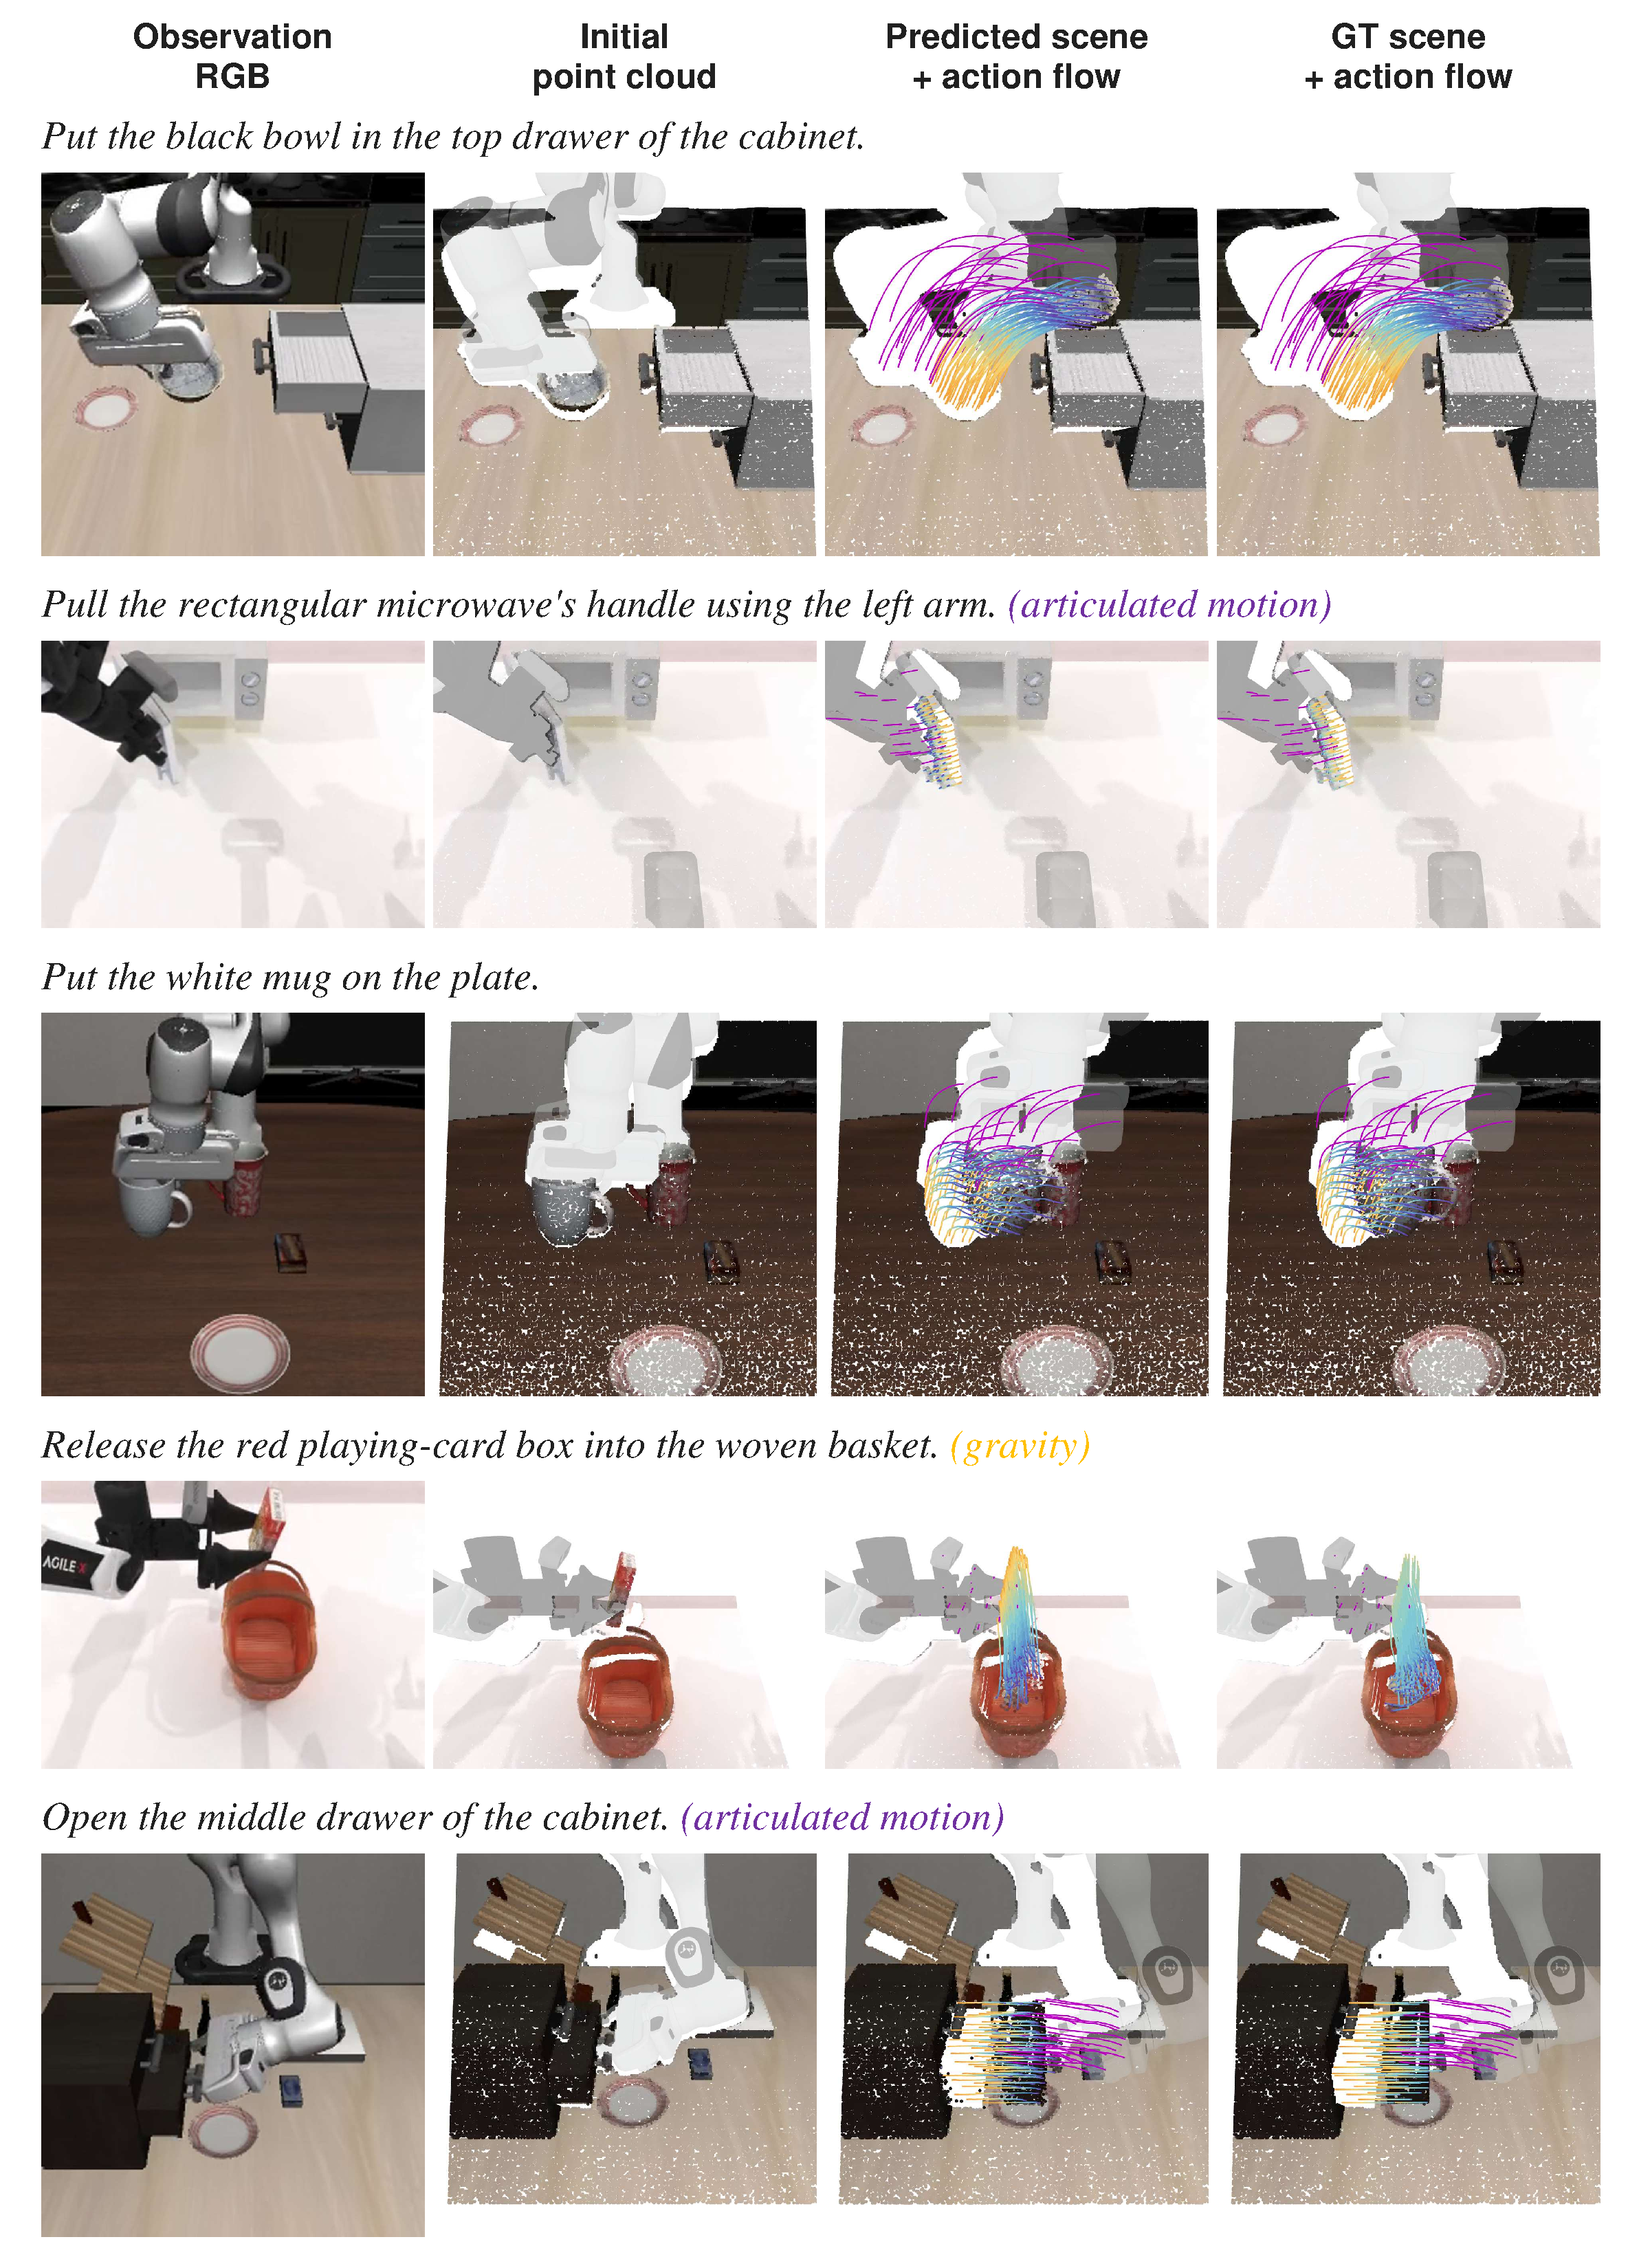
\includegraphics[width=\linewidth]{figures/scene_flow_appendix_2.pdf}
    \caption{Additional scene-flow visualizations (2/4): bowl and mug placement,
    articulated motion, and gravity-driven motion after object release.}
    \label{fig:app:scene_flow_2}
\end{minipage}
\end{center}


\begin{center}
\begin{minipage}{\linewidth}
\makeatletter\def\@captype{figure}\makeatother
    \centering
    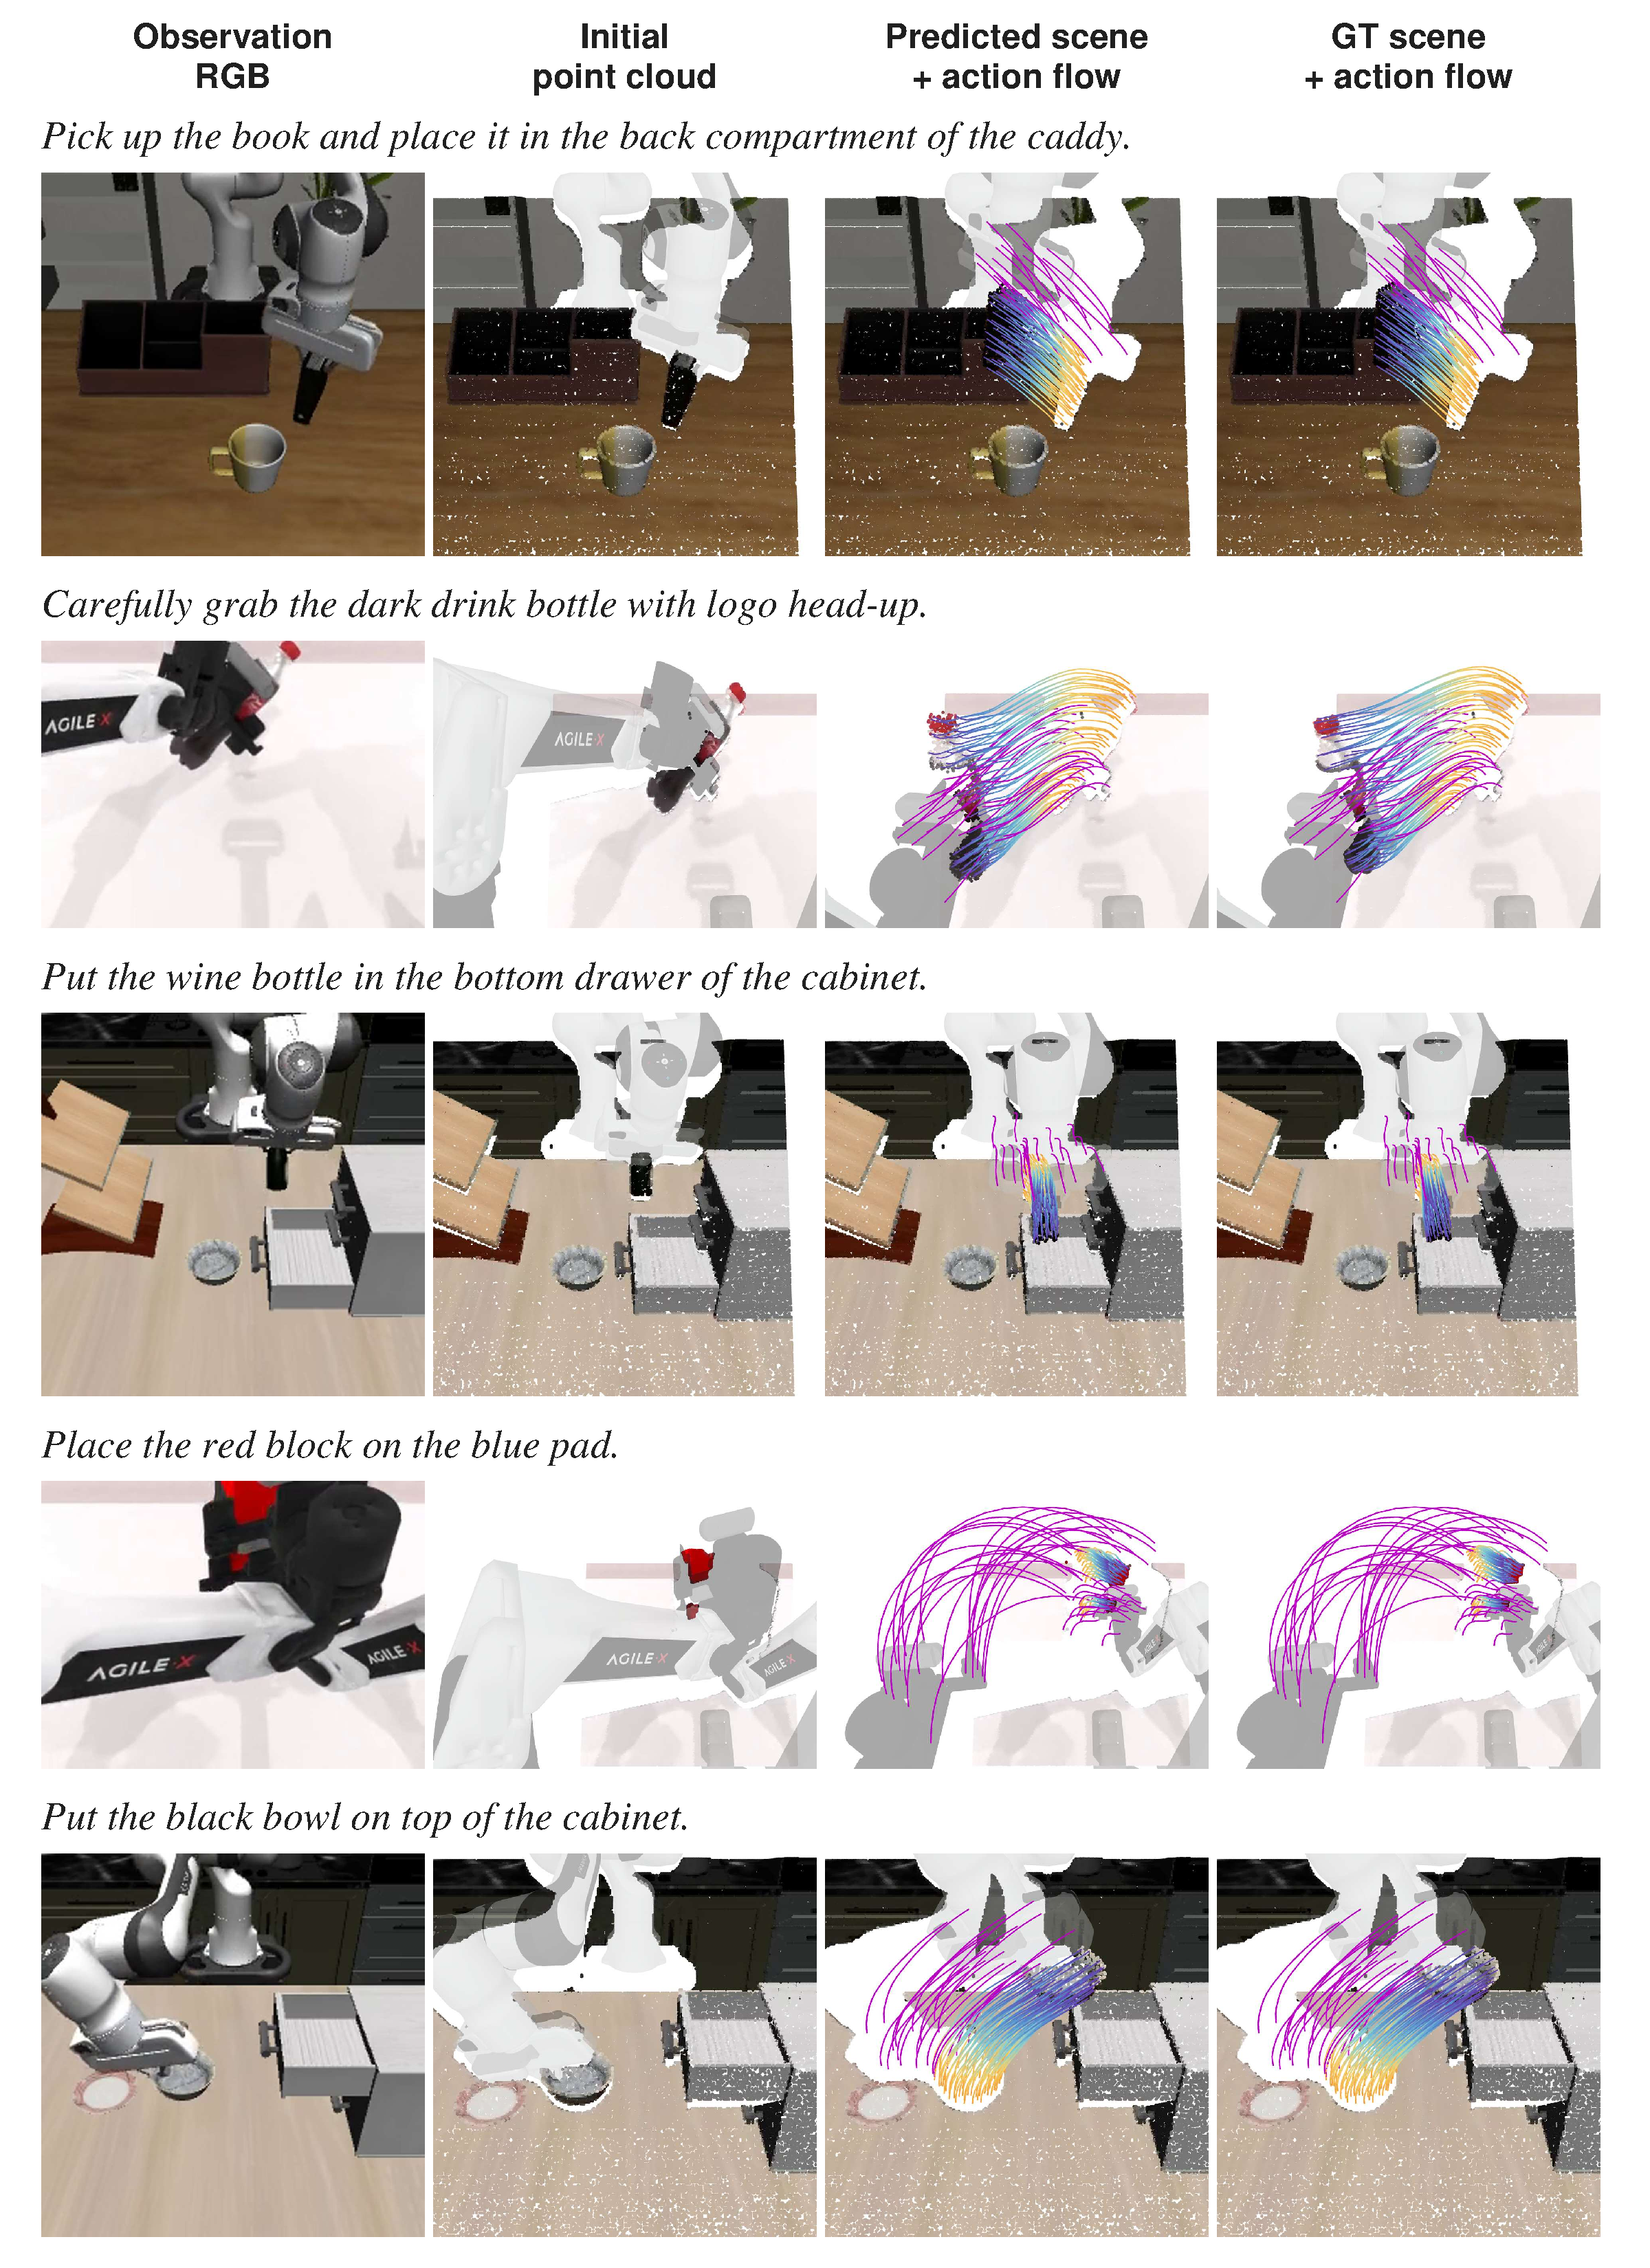
\includegraphics[width=\linewidth]{figures/scene_flow_appendix_3.pdf}
    \caption{Additional scene-flow visualizations (3/4): book, bottle, block,
    and bowl manipulation across LIBERO and RoboTwin.}
    \label{fig:app:scene_flow_3}
\end{minipage}
\end{center}


\begin{center}
\begin{minipage}{\linewidth}
\makeatletter\def\@captype{figure}\makeatother
    \centering
    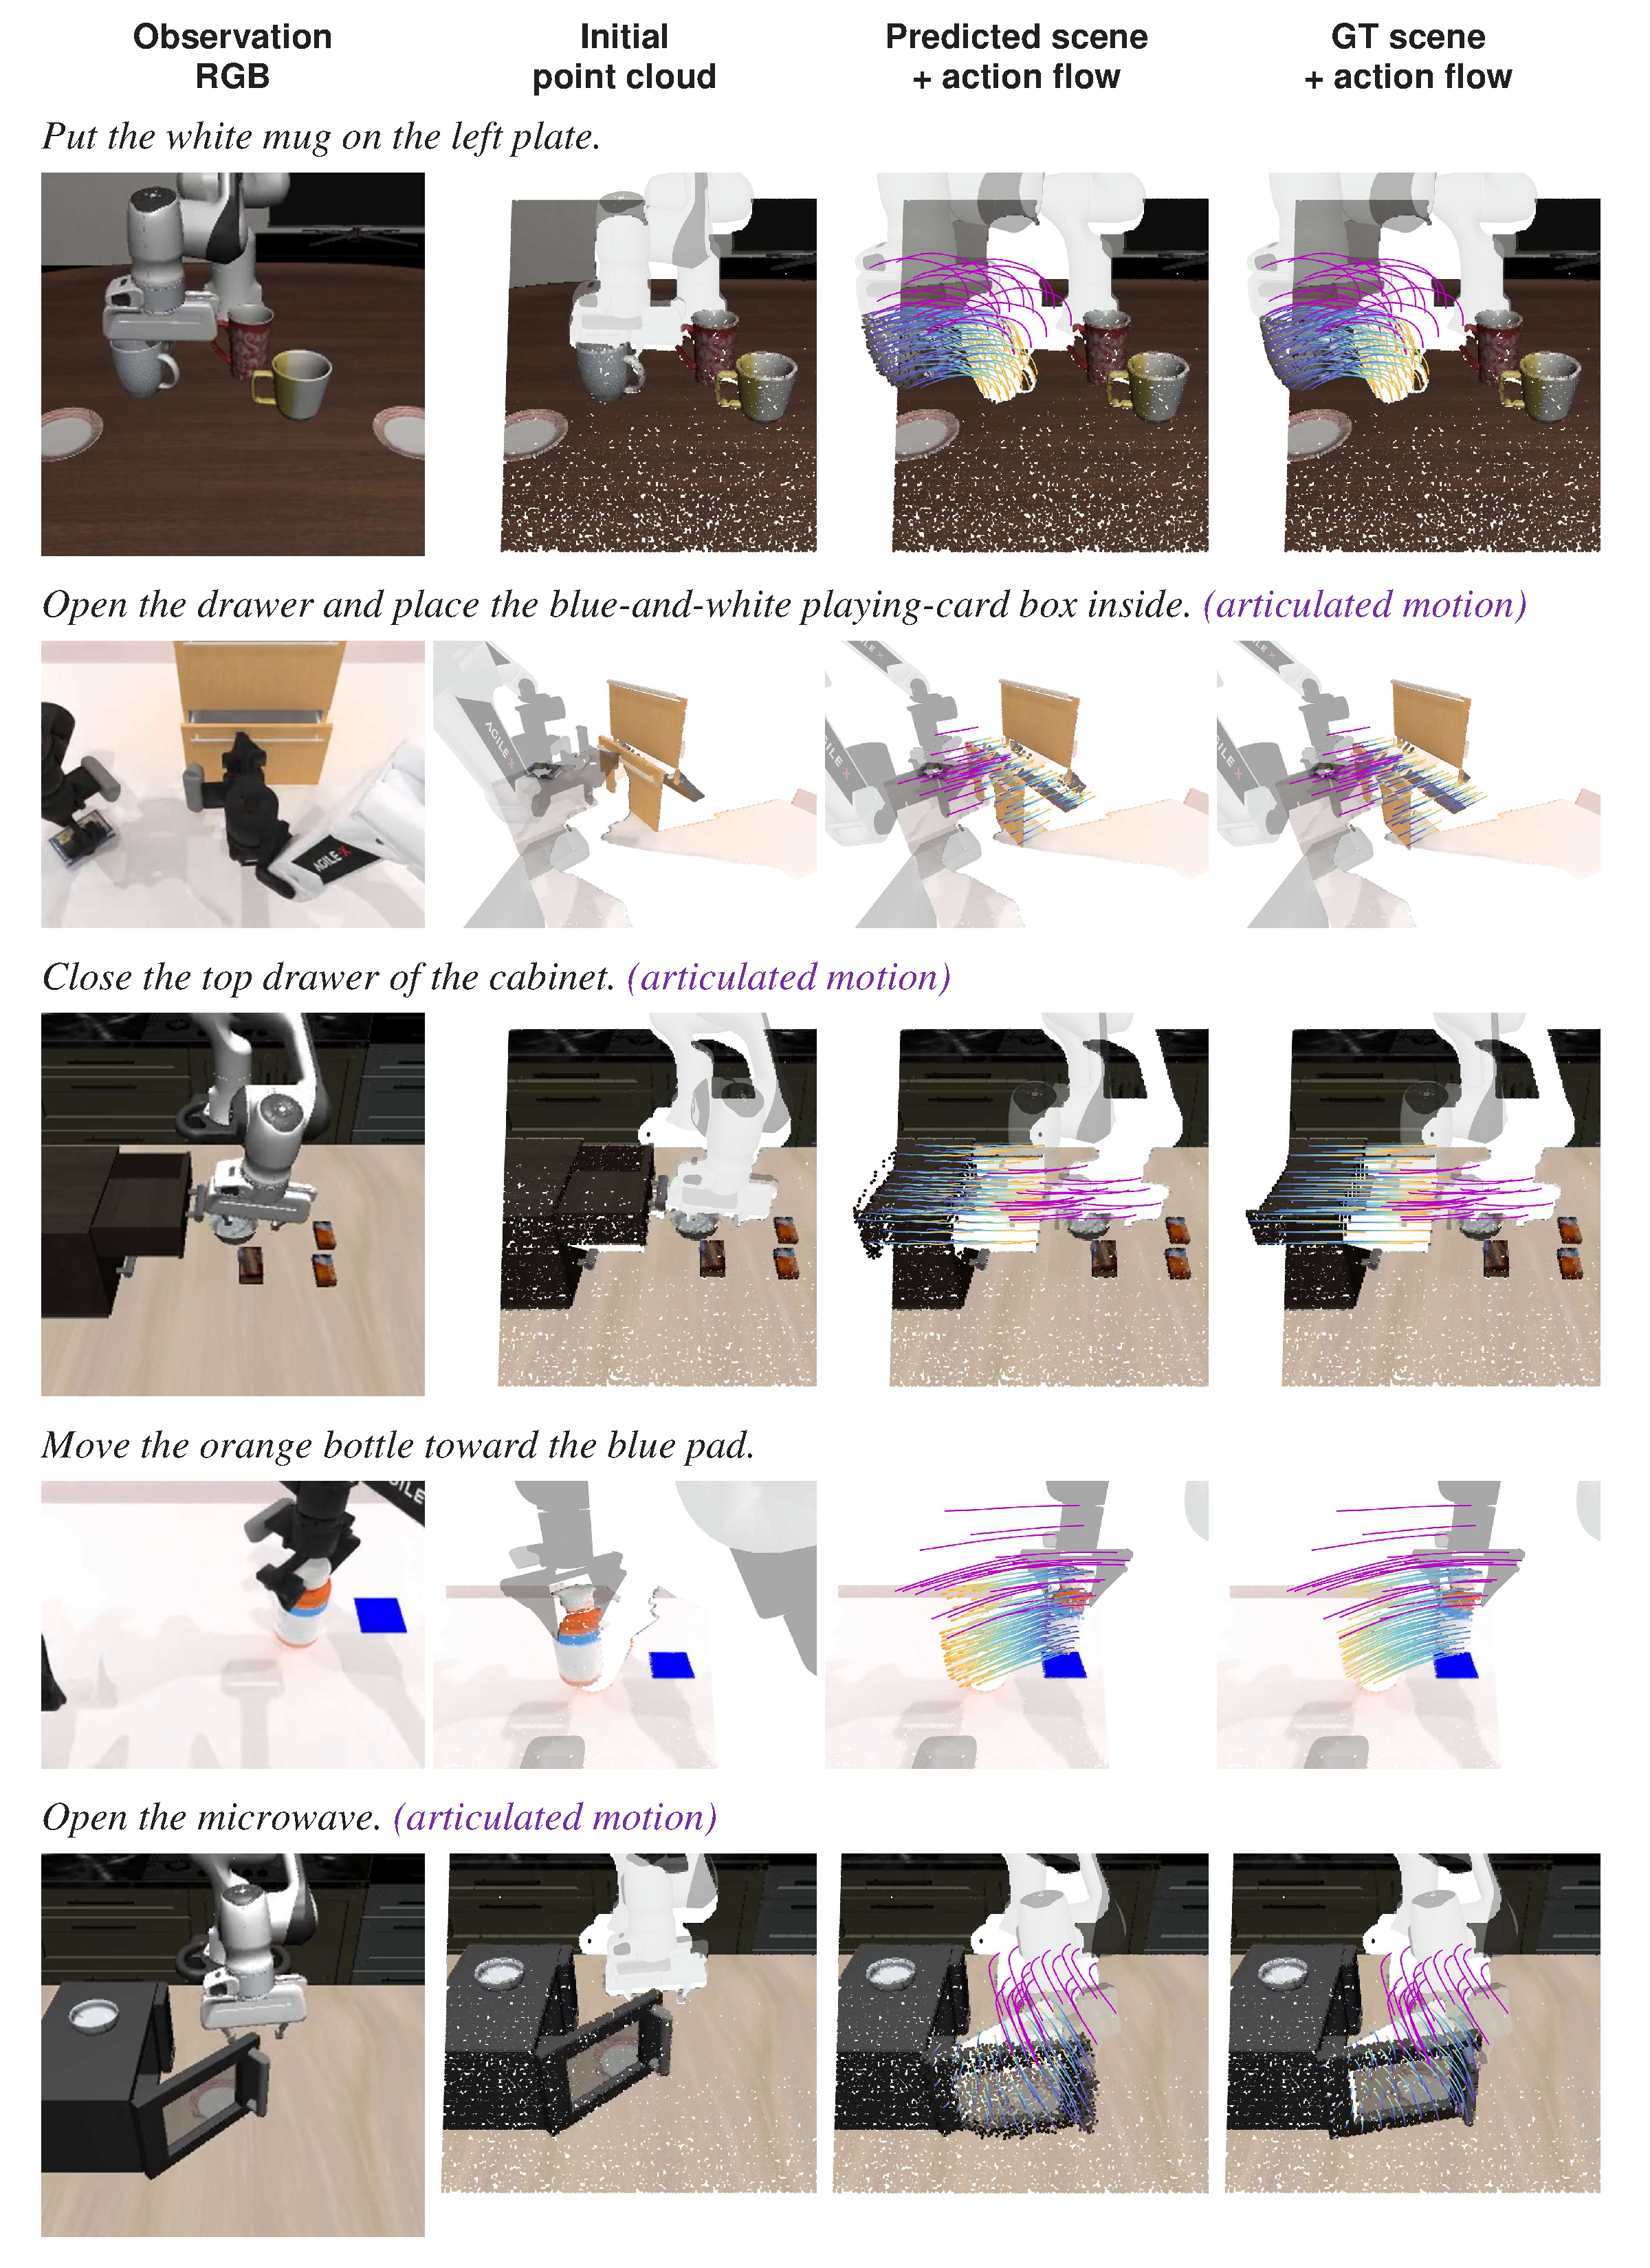
\includegraphics[width=\linewidth]{figures/scene_flow_appendix_4.pdf}
    \caption{Additional scene-flow visualizations (4/4): object placement,
    drawer opening and closing, and microwave opening.}
    \label{fig:app:scene_flow_4}
\end{minipage}
\end{center}


\clearpage
\subsection{Transfer to Real-World Observations}
\label{app:real_scene_flow}

Fig.~\ref{fig:app:real_scene_flow} shows predictions on DROID and RH20T
conditioned on ground-truth gripper trajectories. Despite receiving
scene-flow supervision only from simulation, \method{} captures
action-conditioned scene changes in real environments outside this
supervision distribution. These qualitative results suggest that the
learned interaction dynamics can transfer from simulation to real scenes.
% TODO: Identify the world-model checkpoint and whether each displayed
% episode was used for gripper-flow or other training objectives.

\begin{center}
\begin{minipage}{\linewidth}
\makeatletter\def\@captype{figure}\makeatother
    \centering
    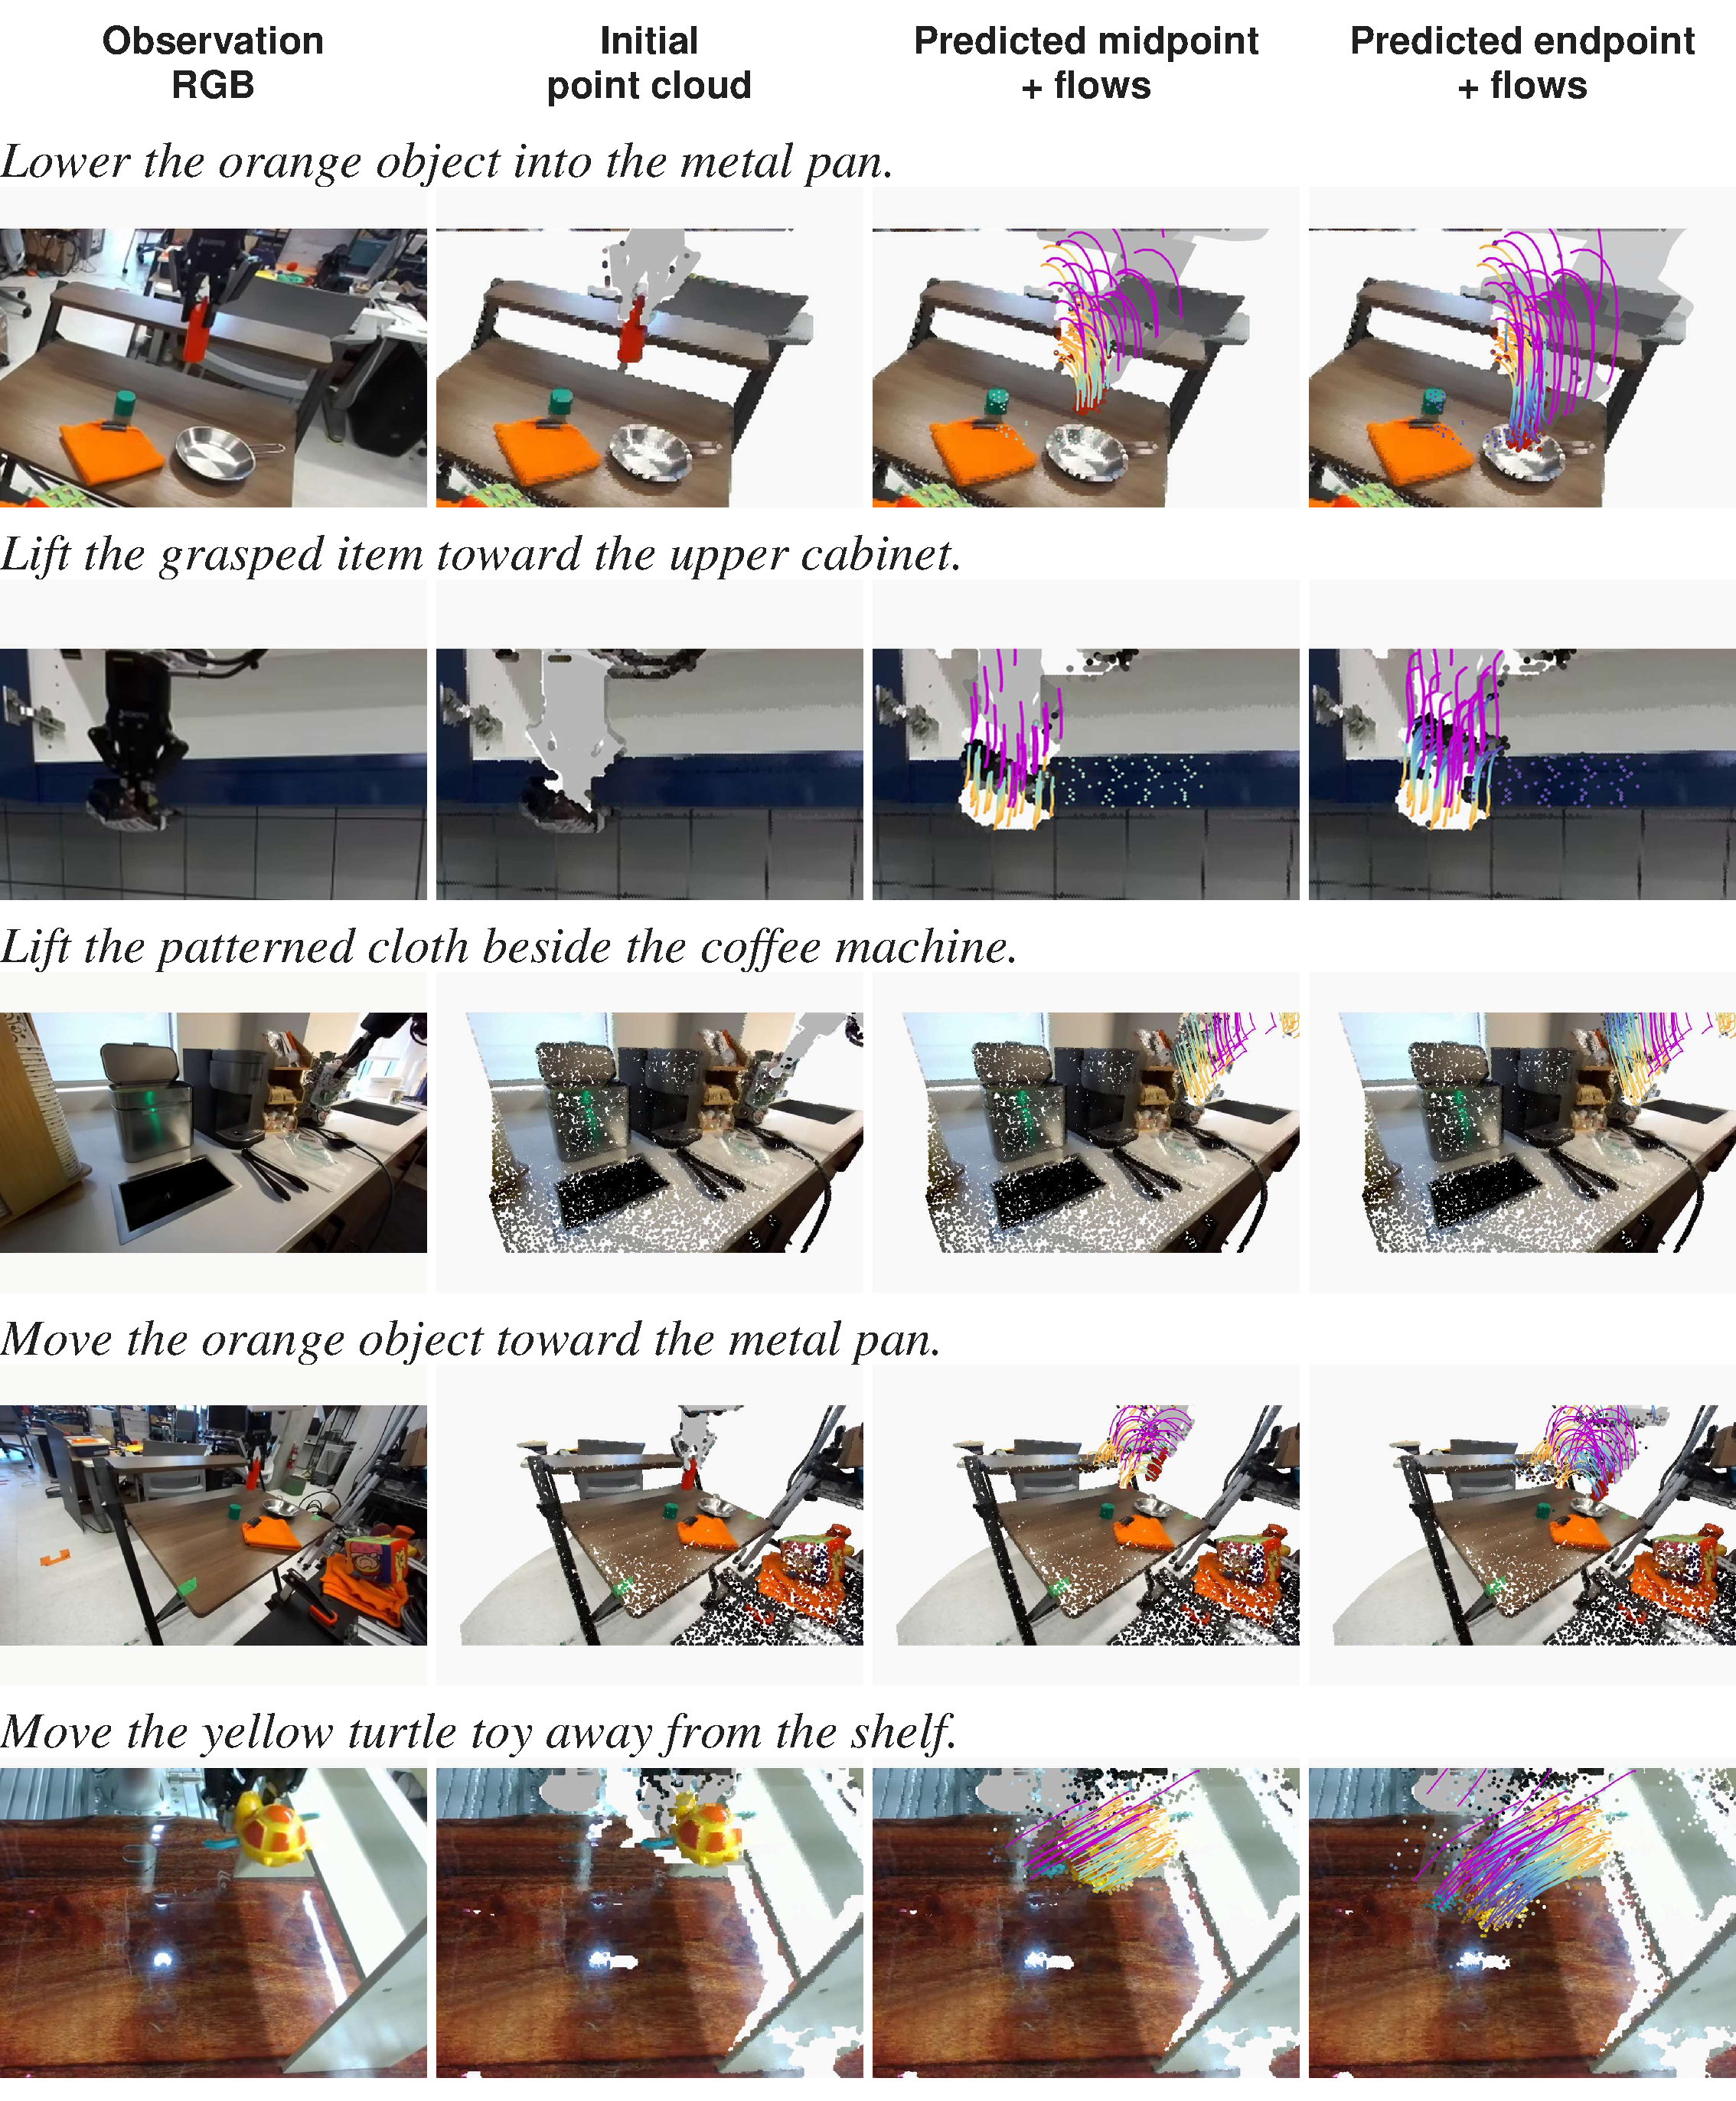
\includegraphics[width=\linewidth]{figures/real_scene_flow_appendix.pdf}
    \caption{\textbf{Zero-shot scene-flow predictions on real-world observations.}
    The first four rows are from DROID and the last is from RH20T.
    Columns show observed RGB, initial points, and predicted midpoint and
    endpoint point clouds with scene trajectories (orange to purple) and
    ground-truth gripper trajectories used for conditioning (magenta).
    No scene-trajectory ground truth is shown.}
    \label{fig:app:real_scene_flow}
\end{minipage}
\end{center}
